\documentclass[a4paper,12pt]{article}
\usepackage[utf8]{inputenc}
\usepackage[margin=1in]{geometry}
\usepackage{amsmath}
\usepackage{graphicx}
\graphicspath{{figures/},{figures/verification_figures},{figures/results_figures},{figures/nearfield_figures}}
\usepackage{tikz}
\usepackage{hyperref}
\hypersetup{
    colorlinks=true,
    linkcolor=blue,
    filecolor=magenta,      
    urlcolor=cyan,
    }
\urlstyle{same}

\renewcommand{\vec}[1]{\boldsymbol{#1}}
\newcommand{\unitvec}[1]{\hat{\vec{#1}}}
\newcommand{\mrm}[1]{\mathrm{#1}}
\newcommand{\diff}{\operatorname{d}\!}
\newcommand{\mat}[1]{\mathbf{#1}}
\newcommand{\unit}[1]{\ensuremath{\,\mrm{#1}}}
\renewcommand{\Re}{\operatorname{Re}}
\renewcommand{\Im}{\operatorname{Im}}

\newcommand{\iu}{\mrm{i}}
\newcommand{\ju}{\mrm{j}}
\newcommand{\eu}{\mrm{e}}
\newcommand{\cu}{\mrm{c}_{0}}
\newcommand{\Ev}{\vec{E}}
\newcommand{\Hv}{\vec{H}}
\newcommand{\Fv}{\vec{F}}
\newcommand{\pv}{\vec{p}}
\newcommand{\rv}{\vec{r}}
\newcommand{\kv}{\vec{k}}
\newcommand{\av}{\vec{a}}
\newcommand{\Zv}{\vec{0}}
\newcommand{\xuv}{\unitvec{x}}
\newcommand{\yuv}{\unitvec{y}}
\newcommand{\zuv}{\unitvec{z}}
\newcommand{\ruv}{\unitvec{r}}
\newcommand{\nuv}{\unitvec{n}}
\newcommand{\tuv}{\unitvec{t}}
\newcommand{\kuv}{\unitvec{k}}
\newcommand{\uuv}{\unitvec{u}}
\newcommand{\rhouv}{\unitvec{\rho}}
\newcommand{\varphiuv}{\unitvec{\varphi}}
\newcommand{\puv}{\unitvec{p}}
\newcommand{\suv}{\unitvec{s}}
\newcommand{\IM}{\mat{I}}
\newcommand{\ZM}{\mat{Z}}
\newcommand{\SM}{\mat{S}}
\newcommand{\TM}{\mat{T}}
\newcommand{\rmat}{\mat{r}}

\newcommand{\thetauv}{\unitvec{\theta}}
\newcommand{\phiuv}{\unitvec{\phi}}

\newcommand{\BesselJ}{\operatorname{J}}

\newcommand{\uv}{\vec{u}}
\newcommand{\vv}{\vec{v}}
\newcommand{\epsm}{\boldsymbol{\epsilon}}
\newcommand{\mum}{\boldsymbol{\mu}}

\usepackage{listings}

\usepackage{xcolor}

\definecolor{codegreen}{rgb}{0,0.6,0}
\definecolor{codegray}{rgb}{0.5,0.5,0.5}
\definecolor{codepurple}{rgb}{0.58,0,0.82}
\definecolor{backcolour}{rgb}{0.95,0.95,0.92}

\lstdefinestyle{mystyle}{
    backgroundcolor=\color{backcolour},   
    commentstyle=\color{codegreen},
    keywordstyle=\color{magenta},
    numberstyle=\tiny\color{codegray},
    stringstyle=\color{codepurple},
    basicstyle=\ttfamily\footnotesize,
    breakatwhitespace=false,         
    breaklines=true,                 
    captionpos=b,                    
    keepspaces=true,                 
    numbers=left,                    
    numbersep=5pt,                  
    showspaces=false,                
    showstringspaces=false,
    showtabs=false,                  
    tabsize=2
}

\lstset{style=mystyle}




\title{Scattering computations using a rotationally symmetric solver
  implemented in open source finite elements}

\author{Daniel Sj\"oberg}

\begin{document}
\maketitle

\begin{abstract}
  We summarize the theory and implementation of an open source solver
  for rotationally symmetric scatterers. The purpose of the code is to
  compute reference solutions for electrically large radome problems.
\end{abstract}


\section{Introduction}



\section{Rotational symmetry}
\label{sec:rotational}

In order to conserve the computational size of the problem to be
simulated, we may consider a rotationally symmetric structure, which
in principle converts the problem from 3D to 2D. This is a huge saving
in computational complexity, but since an arbitrary excitation
involves all azimuthal modes, we typically need to solve for very many
modes and synthesize the resulting solution as a superposition of the
modes, which renders the name ``2.5D'' for the resulting dimensional
complexity of the problem. The number of modes necessary is determined
from the Wiscombe criterion \cite{Wiscombe1980}, which in its most
restrictive form is
\begin{equation}
  N > ka + 4.05(ka)^{3} + 2
\end{equation}
where $a$ is the radius of the scattering region, and
$k = 2\pi/\lambda$ is the free space wavenumber. In order to reduce
the number of modes solved for in order to obtain quick test cases, we
can require symmetry from the excitation. Typically, we may restrict
the antenna to radiate along the axis of rotational symmetry
($z$-axis) with linear or circular polarization, or have a plane wave
incident along the axis, requiring only two azimuthal modes
($m=\pm1$).


\subsection{Representation in cylindrical coordinates}

For a rotationally symmetric structure, it is beneficial to express
the fields in cylindrical coordinates $(\rho,\varphi,z)$ as
\begin{align}
  \Ev(\rv) &= \sum_{m=-\infty}^{\infty} \left[E_{\rho}^{(m)}(\rho,z)\rhouv + E_{\varphi}^{(m)}(\rho,z)\varphiuv + E_{z}^{(m)}(\rho,z)\zuv \right] \eu^{-\ju m\varphi} \\
  \Hv(\rv) &= \sum_{m=-\infty}^{\infty} \left[H_{\rho}^{(m)}(\rho,z)\rhouv + H_{\varphi}^{(m)}(\rho,z)\varphiuv + H_{z}^{(m)}(\rho,z)\zuv \right] \eu^{-\ju m\varphi}
\end{align}
This representation is valid for any structure, but for a rotationally
symmetric structure there is no coupling between the azimuthal modes
and we may consider each mode index $m$ separately in Maxwell's
equations. The curl operation can be written in cylindrical
coordinates as
\begin{equation}
  \nabla\times\Ev = \rhouv\left(\frac{1}{\rho}\frac{\partial E_{z}}{\partial\varphi} - \frac{\partial E_{\varphi}}{\partial z}\right) + \varphiuv\left(\frac{\partial E_{\rho}}{\partial z} - \frac{\partial E_{z}}{\partial\rho}\right) + \zuv\left( \frac{1}{\rho}\frac{\partial}{\partial\rho}(\rho E_{\varphi}) - \frac{1}{\rho}\frac{\partial E_{\rho}}{\partial\varphi}\right)
\end{equation}
Maxwell's equations in isotropic space, $\nabla\times\Ev =
-\ju\omega\mu\Hv$ and $\nabla\times\Hv =
\ju\omega\epsilon\Ev$, can then be written
\begin{align}
  -\frac{\ju m}{\rho}E_{z}^{(m)} - \frac{\partial E_{\varphi}^{(m)}}{\partial z} &= -\ju\omega\mu H_{\rho}^{(m)} & 
  -\frac{\ju m}{\rho}H_{z}^{(m)} - \frac{\partial H_{\varphi}^{(m)}}{\partial z} &= \ju\omega\epsilon E_{\rho}^{(m)} \label{eq:Maxwellrho} \\
  \frac{\partial E_{\rho}^{(m)}}{\partial z} - \frac{\partial E_{z}^{(m)}}{\partial\rho} &= -\ju\omega\mu H_{\varphi}^{(m)} & 
  \frac{\partial H_{\rho}^{(m)}}{\partial z} - \frac{\partial H_{z}^{(m)}}{\partial\rho} &= \ju\omega\epsilon E_{\varphi}^{(m)} \label{eq:Maxwellvarphi} \\
  \frac{1}{\rho}\frac{\partial}{\partial\rho}(\rho E_{\varphi}^{(m)}) + \frac{\ju m}{\rho}E_{\rho}^{(m)} &= -\ju\omega\mu H_{z}^{(m)} &
  \frac{1}{\rho}\frac{\partial}{\partial\rho}(\rho H_{\varphi}^{(m)}) + \frac{\ju m}{\rho}H_{\rho}^{(m)} &= \ju\omega\epsilon E_{z}^{(m)} \label{eq:Maxwellz}
\end{align}
It is seen that only for $m=0$ do these equations split into an
in-plane electric field mode
$(E_{\rho}^{(0)},E_{z}^{(0)},H_{\varphi}^{(0)})$, and an out-of-plane
electric field mode
$(E_{\varphi}^{(0)},H_{\rho}^{(0)},H_{z}^{(0)})$. For $m\neq0$, we
need to solve for all field components.

As noted in \cite[p. 906]{vanBladel2007}, for a field continuous on
the axis $\rho=0$ we must have
\begin{align}
  E_{\rho}^{(m)}(0,z) = E_{\varphi}^{(m)}(0,z) &= 0 && \text{for $m = 0$} \label{eq:axialcond_a} \\
  E_{z}^{(m)}(0,z) = E_{\varphi}^{(m)}(0,z) + \ju m E_{\rho}(^{(m)}(0,z) &= 0 && \text{for $m = \pm 1$} \label{eq:axialcond_b} \\
  E_{\rho}^{(m)}(0,z) = E_{z}^{(m)}(0,z) = E_{\varphi}^{(m)}(0,z) &= 0 && \text{for $|m| > 1$} \label{eq:axialcond_c}
\end{align}
These equations correspond to Dirichlet boundary conditions on the
axis $\rho=0$ when solving the equations in the domain
$\rho>0$. However, in a finite element formulation, they are also
enforced directly by the weak formulation, and do not require
implementation as explicit Dirichlet conditions.


\subsection{Finite element formulation}

The general finite element formulation in an isotropic medium is
(where $\Ev$ is the scattered field and $\Ev_{\mrm{b}}$ is the
excitation in terms of a background field)
\begin{multline}
  \int_{\Omega} \left\{ - \mu_{\mrm{r}}^{-1}[\nabla\times(\Ev+\Ev_{\mrm{b}})]\cdot(\nabla\times\vv^{*}) + k_{0}^{2}\epsilon_{\mrm{r}} (\Ev+\Ev_{\mrm{b}})\cdot\vv^{*} \right\} \diff V \\
  + \int_{\Omega_{\mrm{pml}}} \left\{ -[\mum_{\mrm{r,pml}}^{-1}\cdot(\nabla\times\Ev)]\cdot(\nabla\times\vv^{*}) + k_{0}^{2}[\epsm_{\mrm{r,pml}}\cdot\Ev]\cdot\vv^{*} \right\} \diff V = 0
\end{multline}
Taking into account that the background field satisfies
$\int_{\Omega}\mu_{\mrm{r,b}}^{-1} (\nabla\times\Ev_{\mrm{b}}) \cdot
(\nabla\times\vv^{*}) \diff V = \int_{\Omega}
\epsilon_{\mrm{r,b}}k_{0}^{2}\Ev_{\mrm{b}}\cdot\vv^{*} \diff V$, this
can also be written
\begin{multline}
  \int_{\Omega} \left\{ - \mu_{\mrm{r}}^{-1}(\nabla\times\Ev)\cdot(\nabla\times\vv^{*}) + k_{0}^{2}\epsilon_{\mrm{r}}\Ev\cdot\vv^{*} \right\} \diff V + \int_{\Omega} k_{0}^{2} (\epsilon_{\mrm{r}}-\mu_{\mrm{r}}^{-1}\mu_{\mrm{r,b}}\epsilon_{\mrm{r,b}}) \Ev_{\mrm{b}}\cdot\vv^{*} \diff V \\
  + \int_{\Omega_{\mrm{pml}}} \left\{ -[\mum_{\mrm{r,pml}}^{-1}\cdot(\nabla\times\Ev)]\cdot(\nabla\times\vv^{*}) + k_{0}^{2} [\epsm_{\mrm{r,pml}}\cdot\Ev]\cdot\vv^{*} \right\} \diff V = 0
\end{multline}
where it is seen that the background field acts as a source term in
regions where
$\epsilon_{\mrm{r}}-\mu_{\mrm{r}}^{-1}\mu_{\mrm{r,b}}\epsilon_{\mrm{r,b}}
\neq 0$. Often, we are dealing with non-magnetic materials and the
expression simplifies to
$\epsilon_{\mrm{r}}-\epsilon_{\mrm{r,b}}$. Also, the background
material is often taken as vacuum, that is,
$\epsilon_{\mrm{r,b}} = 1$.

Considering the curl operation on one azimuthal mode, we may define
the differential operator $\nabla_{m}$
\begin{multline}
  \nabla_{m}\times\Ev^{(m)} = \eu^{\ju m\varphi}\nabla\times(\Ev^{(m)}\eu^{-\ju m\varphi}) \\
  = \rhouv\left(-\frac{\ju m}{\rho}E_{z}^{(m)} - \frac{\partial E_{\varphi}^{(m)}}{\partial z}\right) + \varphiuv\left(\frac{\partial E_{\rho}^{(m)}}{\partial z} - \frac{\partial E_{z}^{(m)}}{\partial\rho}\right) + \zuv\left( \frac{1}{\rho}\frac{\partial}{\partial\rho}(\rho E_{\varphi}^{(m)}) + \frac{\ju m}{\rho}E_{\rho}^{(m)}\right)
\end{multline}
Using test functions
$\vv(\rv) = \sum_{m=-\infty}^{\infty}\vv^{(m)}(\rho,z)\eu^{-\ju
  m\varphi}$, we find that the integral over $\varphi$ is non-zero
only when corresponding azimuthal modes are used for both the electric
field and the test function, hence we have the two-dimensional
formulation
\begin{multline}
  \int_{\Omega} \left\{ - \mu_{\mrm{r}}^{-1}(\nabla_{m}\times\Ev^{(m)})\cdot(\nabla_{m}\times\vv^{(m),*}) + k_{0}^{2}\epsilon_{\mrm{r}}\Ev^{(m)}\cdot\vv^{(m),*} \right\} \rho\diff\rho\diff z \\
  + \int_{\Omega} k_{0}^{2} (\epsilon_{\mrm{r}}-\mu_{\mrm{r}}^{-1}\mu_{\mrm{r,b}}\epsilon_{\mrm{r,b}}) \Ev_{\mrm{b}}^{(m)}\cdot\vv^{(m),*} \rho\diff\rho\diff z \\
  + \int_{\Omega_{\mrm{pml}}} \left\{ -[\mum_{\mrm{r,pml}}^{-1}\cdot(\nabla_{m}\times\Ev^{(m)})]\cdot(\nabla_{m}\times\vv^{(m),*}) + k_{0}^{2} \epsm_{\mrm{r,pml}}\cdot\Ev^{(m)}\cdot\vv^{(m),*} \right\} \rho\diff\rho\diff z = 0
\end{multline}
The boundary condition $\nuv\times(\Ev + \Ev_{\mrm{b}}) = \Zv$ on
metal boundaries can be enforced by the functional
\begin{equation}
  \frac{\alpha}{h}\int_{\Gamma_{\mrm{pec}}} [\nuv\times(\Ev + \Ev_{\mrm{b}})] \cdot [\nuv\times\vv^{(m),*}] \diff\ell
\end{equation}
where $h$ is the triangle diameter and $\alpha=10$ is a tuning
parameter. 
Finally, to prescribe an antenna excitation $\Ev_{\mrm{a}}$ on a
surface representing an antenna, we use a similar functional
\begin{equation}
  \frac{\alpha}{h}\int_{\Gamma_{\mrm{ant}}} [\nuv\times(\Ev + \Ev_{\mrm{b}} - \Ev_{\mrm{a}})] \cdot [\nuv\times\vv^{(m),*}] \diff\ell
\end{equation}
This treats the antenna surface as a metal boundary with reflection
coefficient $-1$ for the background field. In total, our weak
formulation is then
\begin{multline}
  \int_{\Omega} \left\{ - \mu_{\mrm{r}}^{-1}(\nabla_{m}\times\Ev^{(m)})\cdot(\nabla_{m}\times\vv^{(m),*}) + k_{0}^{2} \epsilon_{\mrm{r}}\Ev^{(m)}\cdot\vv^{(m),*} \right\} \rho\diff\rho\diff z \\
  + \int_{\Omega} k_{0}^{2} (\epsilon_{\mrm{r}}-\mu_{\mrm{r}}^{-1}\mu_{\mrm{r,b}}\epsilon_{\mrm{r,b}}) \Ev_{\mrm{b}}^{(m)}\cdot\vv^{(m),*} \rho\diff\rho\diff z \\
  + \frac{\alpha}{h}\int_{\Gamma_{\mrm{pec}}} [\nuv\times(\Ev + \Ev_{\mrm{b}})] \cdot [\nuv\times\vv^{(m),*}] \diff\ell 
  + \frac{\alpha}{h}\int_{\Gamma_{\mrm{ant}}} [\nuv\times(\Ev + \Ev_{\mrm{b}} - \Ev_{\mrm{a}})] \cdot [\nuv\times\vv^{(m),*}] \diff\ell \\
  + \int_{\Omega_{\mrm{pml}}} \left\{ -[\mum_{\mrm{r,pml}}^{-1}\cdot(\nabla_{m}\times\Ev^{(m)})]\cdot(\nabla_{m}\times\vv^{(m),*}) + k_{0}^{2}[\epsm_{\mrm{r,pml}}\cdot\Ev^{(m)}]\cdot\vv^{(m),*} \right\} \rho\diff\rho\diff z = 0
\end{multline}
The finite element is chosen as a mixed element, representing
$(E_{\rho},E_{z})$ with curl conforming first kind Nédélec (N1curl),
and $E_{\varphi}$ with node based Lagrange elements, both of degree 3.

\subsection{Perfectly matched layer}

A perfectly matched layer (PML) region is used to absorb the outgoing
scattered field. We follow the dolfinx v0.7 demo on axisymmetric
scattering,\footnote{\url{https://docs.fenicsproject.org/dolfinx/main/python/demos/demo_axis.html}}
and consider a spherical region with stretched cylindrical coordinates
$\rho'(\rho,z)$, $z'(\rho,z)$, and $\varphi'=\varphi$. The coordinate
transformation has the Jacobian
\begin{equation}
  \mat{J} = \mat{A}^{-1} = \nabla\rv'(\rv) =
  \begin{pmatrix}
    \frac{\partial\rho'}{\partial\rho} & \frac{\partial z'}{\partial\rho} & 0 \\
    \frac{\partial\rho'}{\partial z} & \frac{\partial z'}{\partial z} & 0 \\
    0 & 0 & \frac{\rho'}{\rho}\frac{\partial\varphi'}{\partial\varphi}
  \end{pmatrix}
\end{equation}
and the PML material parameters are (with
$A=\operatorname{det}(\mat{A})$) 
\begin{align}
  \epsm_{\mrm{r,pml}} = A^{-1} \mat{A} \boldsymbol{\epsilon}_{\mrm{b}} \mat{A}^{\mrm{T}} \\
  \mum_{\mrm{r,pml}} = A^{-1} \mat{A} \boldsymbol{\mu}_{\mrm{b}} \mat{A}^{\mrm{T}} 
\end{align}
We consider stretching with a polynomial profile such that
\cite[p. 663]{Taflove+etal2004}
\begin{align}
  \rho' &= \rho\left( 1 - \ju \frac{(n+1)\ln(1/R_{0})}{2k_{0}(r_{\mrm{pml}} - r_{\mrm{dom}})} \left(\frac{r-r_{\mrm{dom}}}{r_{\mrm{pml}} - r_{\mrm{dom}}}\right)^{n}\right) \\
  z' &= z\left( 1 - \ju \frac{(n+1)\ln(1/R_{0})}{2k_{0}(r_{\mrm{pml}} - r_{\mrm{dom}})} \left(\frac{r-r_{\mrm{dom}}}{r_{\mrm{pml}} - r_{\mrm{dom}}}\right)^{n}\right) 
\end{align}
where $R_{0}$ is the desired (amplitude scale) reflection coefficient
at normal incidence, $n$ is the polynomial order, and
$r = \sqrt{\rho^{2} + z^{2}}$. Suitable choices seem to be
$R_{0} = 10^{-10}$ and $n=3$.

Another option, which allows for structures parallel to the $z$-axis
extending into the PML (and hence considered infinite in this
direction), would be
\begin{align}
  \rho' &= \rho\left( 1 - \ju \frac{(n+1)\ln(1/R_{0})}{2k_{0}(\rho_{\mrm{pml}} - \rho_{\mrm{dom}})} \left(\frac{\rho-\rho_{\mrm{dom}}}{\rho_{\mrm{pml}} - \rho_{\mrm{dom}}}\right)^{n}\right) && \rho_{\mrm{dom}} < \rho < \rho_{\mrm{pml}} \\
  z' &= z\left( 1 - \ju \frac{(n+1)\ln(1/R_{0})}{2k_{0}(z_{\mrm{pml,t}} - z_{\mrm{dom,t}})} \left(\frac{z-z_{\mrm{dom,t}}}{z_{\mrm{pml,t}} - z_{\mrm{dom,t}}}\right)^{n}\right) && z_{\mrm{dom,t}} < z < z_{\mrm{pml,t}} \\
  z' &= z\left( 1 - \ju \frac{(n+1)\ln(1/R_{0})}{2k_{0}(z_{\mrm{dom,b}} - z_{\mrm{pml,b}})} \left(\frac{z_{\mrm{dom,b}}-z}{z_{\mrm{dom,b}} - z_{\mrm{pml,b}}}\right)^{n}\right) && z_{\mrm{pml,b}} < z < z_{\mrm{dom,b}} 
\end{align}
and unstretched coordinates otherwise. In the overlap regions, both
$\rho'$ and $z'$ are stretched by the formulas above. We can write a
stretching function (note the use of the absolute value in order to
have positive quantities regardless of the sign of
$x_{\mrm{pml}}-x_{\mrm{dom}}$)
\begin{equation}
  s(x,x_{\mrm{dom}},x_{\mrm{pml}}) = 1 - \ju\frac{(n+1)\ln(1/R_{0})}{2k_{0}|x_{\mrm{pml}} - x_{\mrm{dom}}|} \left(\frac{x-x_{\mrm{dom}}}{x_{\mrm{pml}} - x_{\mrm{dom}}}\right)^{n}
\end{equation}
where $x$ denotes the coordinate normal to the PML, with
$x_{\mrm{dom}}$ and $x_{\mrm{pml}}$ denoting the coordinates at the
end of the domain and the end of the PML, respectively. Hence, a
spherical PML has
\begin{align}
  \rho' &= \rho s(r,r_{\mrm{dom}},r_{\mrm{pml}}) && r_{\mrm{dom}} < r < r_{\mrm{pml}} \\
  z' &= z s(r,r_{\mrm{dom}},r_{\mrm{pml}}) && r_{\mrm{dom}} < r < r_{\mrm{pml}}
\end{align}
with $r = \sqrt{\rho^{2} + z^{2}}$, whereas a cylindrical PML has
\begin{align}
  \rho' &= \rho s(\rho,\rho_{\mrm{dom}},\rho_{\mrm{pml}}) && \rho_{\mrm{dom}} < \rho < \rho_{\mrm{pml}} \\
  z' &= z s(z,z_{\mrm{dom,t}},z_{\mrm{pml,t}}) && z_{\mrm{dom,t}} < z < z_{\mrm{pml,t}} \\
  z' &= z s(z,z_{\mrm{dom,b}},z_{\mrm{pml,b}}) && z_{\mrm{pml,t}} < z < z_{\mrm{dom,t}} 
\end{align}
We note that this is not strictly the correct scaling since $s$
depends on the coordinates, we should have
$s=\partial \rho'/\partial\rho$ etc. However, it seems to work in
practice.

\section{Plane wave in cylindrical coordinates}
\label{sec:planewave}

An incident plane wave is described by
\begin{equation}
  \Ev_{\mrm{b}}(\rv) = \Ev_{0}\eu^{-\ju\kv\cdot\rv}
\end{equation}
where
\begin{equation}
  \kv = k(\xuv\sin\theta\cos\phi + \yuv\sin\theta\sin\phi + \zuv\cos\theta)
\end{equation}
The cartesian unit vectors can be written in terms of the cylindrical as
\begin{align}
  \xuv &= \rhouv\cos\varphi - \varphiuv\sin\varphi \\
  \yuv &= \rhouv\sin\varphi + \varphiuv\cos\varphi \\
  \zuv &= \zuv
\end{align}
implying
\begin{equation}
  \kv\cdot\rv = k\rho\sin\theta(\cos\phi\cos\varphi + \sin\phi\sin\varphi) + kz\cos\theta 
  = k\rho\sin\theta\cos(\varphi-\phi) + kz\cos\theta
\end{equation}
Using the Jacobi-Anger expansion
\begin{equation}
  \eu^{\ju z\cos\varphi} = \sum_{n=-\infty}^{\infty}\ju^{n}\BesselJ_{n}(z)\eu^{\ju n\varphi}
\end{equation}
we can then write
\begin{equation}
  \eu^{-\ju\kv\cdot\rv} = \eu^{-\ju k\rho\sin\theta\cos(\varphi-\phi)}\eu^{-\ju kz\cos\theta} = \eu^{-\ju kz\cos\theta} \sum_{n=-\infty}^{\infty}(-\ju)^{n}\BesselJ_{n}(k\rho\sin\theta)\eu^{-\ju n(\varphi-\phi)}
\end{equation}
The polarization of the wave is
\begin{equation}
  \Ev_{0} = \thetauv E_{\theta} + \phiuv E_{\phi}
\end{equation}
where the unit vectors are
\begin{multline}
  \thetauv = \cos\theta\cos\phi\xuv + \cos\theta\sin\phi\yuv - \sin\theta\zuv \\
  = \cos\theta(\cos\phi\cos\varphi + \sin\phi\sin\varphi)\rhouv + \cos\theta(-\cos\phi\sin\varphi + \sin\phi\cos\varphi)\varphiuv - \sin\theta\zuv \\
  = \cos\theta\cos(\varphi-\phi)\rhouv - \cos\theta\sin(\varphi-\phi)\varphiuv - \sin\theta\zuv
\end{multline}
and
\begin{multline}
  \phiuv = -\sin\phi\xuv + \cos\phi\yuv = (-\sin\phi\cos\varphi + \cos\phi\sin\varphi)\rhouv + (\sin\phi\sin\varphi + \cos\phi\cos\varphi)\varphiuv \\
  = \sin(\varphi-\phi)\rhouv + \cos(\varphi-\phi)\varphiuv
\end{multline}
Using Euler's formula we have
\begin{equation}
  \cos(\varphi-\phi) = \frac{\eu^{\ju(\varphi-\phi)}+\eu^{-\ju(\varphi-\phi)}}{2} \quad\text{and}\quad \sin(\varphi-\phi) = \frac{\eu^{\ju(\varphi-\phi)}-\eu^{-\ju(\varphi-\phi)}}{2\ju}
\end{equation}
and the final version of the plane wave expansion is
\begin{multline}
  \Ev_{0}\eu^{-\ju\kv\cdot\rv} = E_{\theta}\eu^{-\ju kz\cos\theta} \Bigg\{ \left[ \sum_{n=-\infty}^{\infty}(-\ju)^{n}\BesselJ_{n}(k\rho\sin\theta)\frac{1}{2}(\eu^{-\ju (n-1)(\varphi-\phi)} + \eu^{-\ju (n+1)(\varphi-\phi)}) \right]\cos\theta\rhouv \\
  + \left[ \sum_{n=-\infty}^{\infty}(-\ju)^{n}\BesselJ_{n}(k\rho\sin\theta) \frac{1}{2\ju}(\eu^{-\ju (n-1)(\varphi-\phi)} - \eu^{-\ju (n+1)(\varphi-\phi)}) \right](-\cos\theta)\varphiuv \\
  + \left[ \sum_{n=-\infty}^{\infty}(-\ju)^{n}\BesselJ_{n}(k\rho\sin\theta)\eu^{-\ju n(\varphi-\phi)}\right](-\sin\theta)\zuv \Bigg\} \\
  + E_{\phi}\eu^{-\ju kz\cos\theta} \Bigg\{ \left[ \sum_{n=-\infty}^{\infty}(-\ju)^{n}\BesselJ_{n}(k\rho\sin\theta) \frac{1}{2\ju}(\eu^{-\ju (n-1)(\varphi-\phi)} - \eu^{-\ju (n+1)(\varphi-\phi)}) \right]\rhouv \\
  + \left[ \sum_{n=-\infty}^{\infty}(-\ju)^{n}\BesselJ_{n}(k\rho\sin\theta)\frac{1}{2}(\eu^{-\ju (n-1)(\varphi-\phi)} + \eu^{-\ju (n+1)(\varphi-\phi)}) \right] \varphiuv \Bigg\}
\end{multline}
Rewriting in terms of azimuthal modes, we find
\begin{multline}
  \Ev_{0}\eu^{-\ju\kv\cdot\rv} = E_{\theta}\eu^{-\ju kz\cos\theta} \Bigg\{ \sum_{n=-\infty}^{\infty} \frac{1}{2}\left[ (-\ju)^{n+1}\BesselJ_{n+1}(k\rho\sin\theta) + (-\ju)^{n-1}\BesselJ_{n-1}(k\rho\sin\theta)\right] \eu^{-\ju n(\varphi-\phi)} \cos\theta\rhouv \\
  + \sum_{n=-\infty}^{\infty} \frac{1}{2\ju}\left[ (-\ju)^{n+1}\BesselJ_{n+1}(k\rho\sin\theta) - (-\ju)^{n-1}\BesselJ_{n-1}(k\rho\sin\theta)\right] \eu^{-\ju n(\varphi-\phi)} (-\cos\theta)\varphiuv \\
  + \sum_{n=-\infty}^{\infty}(-\ju)^{n}\BesselJ_{n}(k\rho\sin\theta)\eu^{-\ju n(\varphi-\phi)} (-\sin\theta)\zuv \Bigg\} \\
  + E_{\phi}\eu^{-\ju kz\cos\theta} \Bigg\{ \sum_{n=-\infty}^{\infty} \frac{1}{2\ju} \left[ (-\ju)^{n+1}\BesselJ_{n+1}(k\rho\sin\theta) - (-\ju)^{n-1}\BesselJ_{n-1}(k\rho\sin\theta)\right] \eu^{-\ju n(\varphi-\phi)} \rhouv \\
  + \sum_{n=-\infty}^{\infty} \frac{1}{2} \left[ (-\ju)^{n+1}\BesselJ_{n+1}(k\rho\sin\theta) + (-\ju)^{n-1}\BesselJ_{n-1}(k\rho\sin\theta) \right] \eu^{-\ju n(\varphi-\phi)} \varphiuv \Bigg\}
  \label{eq:planewave}
\end{multline}
which is our final expression. This expression can also be used to
compute an antenna excitation $\Ev_{\mrm{a}}$: simply evaluate it on
the antenna surface, possibly multiplied by an amplitude taper.

\section{Farfield computations}
\label{sec:farfield}

The far field amplitude from tangential electric and magnetic fields
on a general surface $S$ with outward normal $\nuv$ is
\begin{equation}
  \Fv(\kuv) = \frac{\ju k}{4\pi} \kuv\times \int_{S} \left[ \Ev(\rv)\times\nuv + \eta_{0}\kuv\times(\nuv\times\Hv(\rv)) \right] \eu^{\ju k\kuv\cdot\rv} \diff S
\end{equation}
where $k=\omega/\cu = 2\pi/\lambda$ is the free space wavenumber
(here, $\omega = 2\pi f$ is the angular frequency at ordinary
frequency $f$, $\lambda$ is the vacuum wavelength, and $\cu$ the speed
of light in vacuum, respectively), and $\kuv$ is the observation
direction.  In the specific case of a rotationally symmetric
structure, the surface $S$ is described by a curve $\gamma$ in the
$\rho-z$ plane, and we have $\Fv(\kuv) = \sum_{m}\Fv^{(m)}(\kuv)$ where
\begin{equation}
  \Fv^{(m)}(\kuv) = \frac{\ju k}{4\pi} \kuv\times \int_{\vec{\rho}\in\gamma}\int_{\varphi=0}^{2\pi} \left[ \Ev^{(m)}(\rho,z)\times\nuv + \eta_{0}\kuv\times(\nuv\times\Hv^{(m)}(\rho,z)) \right] \eu^{\ju(k\kuv\cdot\rv-m\varphi)} \rho\diff\varphi\diff\ell
\end{equation}
The integral in the $\varphi$-direction is explicitly computed in
Appendix~\ref{app:farfield}. The result is
\begin{multline}
  \Fv^{(m)}(\theta,\phi) = \thetauv\frac{\ju k}{2}\ju^{m}\eu^{-\ju
    m\phi} \int_{\vec{\rho}\in\gamma} \Big\{ - \left[ C_{m}
    n_{z}E_{\varphi}^{(m)}
    - S_{m} (n_{\rho}E_{z}^{(m)} - n_{z}E_{\rho}^{(m)}) \right] \sin\phi \\
  + \left[ S_{m} n_{z}E_{\varphi}^{(m)}
    + C_{m} (n_{\rho}E_{z}^{(m)} - n_{z}E_{\rho}^{(m)}) \right] \cos\phi \\
  - \eta_{0} \left[ C_{m} n_{z}H_{\varphi}^{(m)}
    - S_{m} (n_{\rho}H_{z}^{(m)} - n_{z}H_{\rho}^{(m)}) \right] \cos\theta\cos\phi \\
  - \eta_{0}\left[ S_{m} n_{z}H_{\varphi}^{(m)}
    + C_{m} (n_{\rho}H_{z}^{(m)} - n_{z}H_{\rho}^{(m)}) \right] \cos\theta\sin\phi \\
  + \eta_{0} A_{m} n_{\rho}H_{\varphi}^{(m)}
  \sin\theta \Big\} \eu^{\ju kz\cos\theta} \rho\diff\ell \\
  + \phiuv \frac{\ju k}{2} \ju^{m}\eu^{-\ju
    m\phi}\int_{\vec{\rho}\in\gamma} \Big\{ - \left[ C_{m}
    n_{z}E_{\varphi}^{(m)}
    - S_{m} (n_{\rho}E_{z}^{(m)} - n_{z}E_{\rho}^{(m)}) \right] \cos\theta\cos\phi \\
  - \left[ S_{m} n_{z}E_{\varphi}^{(m)}
    + C_{m} (n_{\rho}E_{z}^{(m)} - n_{z}E_{\rho}^{(m)}) \right] \cos\theta\sin\phi \\
  + A_{m} n_{\rho}E_{\varphi}^{(m)} \sin\theta \\
  + \eta_{0} \left[ C_{m} n_{z}H_{\varphi}^{(m)}
    - S_{m} (n_{\rho}H_{z}^{(m)} - n_{z}H_{\rho}^{(m)}) \right] \sin\phi \\
  - \eta_{0}\left[ S_{m} n_{z}H_{\varphi}^{(m)} +
    C_{m} (n_{\rho}H_{z}^{(m)} -
    n_{z}H_{\rho}^{(m)}) \right] \cos\phi \Big\} \eu^{\ju kz\cos\theta}
  \rho\diff\ell
\end{multline}
where
\begin{align}
  A_{m} &= \BesselJ_{m}(k\rho\sin\theta) \\
  C_{m} &= \frac{1}{2}\left[ \eu^{\ju\phi}\BesselJ_{m-1}(k\rho\sin\theta) + \eu^{-\ju\phi}\BesselJ_{m+1}(k\rho\sin\theta) \right] \\
  S_{m} &= \frac{\ju}{2}\left[ \eu^{\ju\phi}\BesselJ_{m-1}(k\rho\sin\theta) - \eu^{-\ju\phi}\BesselJ_{m+1}(k\rho\sin\theta) \right]
\end{align}
This integral can be implemented in FEniCSx. It is important to
restrict the evaluations of the Bessel functions to cells adjacent to
the farfield boundary, in order to keep the overhead computations to a
minimum. 


\section{Projection on spherical vector harmonics}
\label{sec:sphericalvectorharmonics}

In order to limit the data needed to be saved from each simulation,
the far field results can be projected on spherical vector harmonics,
which also enables postprocessing of a 3D radiation pattern.
\begin{itemize}
\item State definitions and properties of complex spherical vector harmonics.
\item State integrals projecting on the harmonics.
\item State how expansion coefficients can be used to construct the 3D farfield.
\end{itemize}
\begin{equation}
  \Ev(\rv) = \sum_{n}f_{n}\uv_{n}(k\rv), \quad r>R
\end{equation}
\begin{equation}
  \Fv(\ruv) = -\frac{4\pi}{\ju k}\SM(\ruv,\kuv)\cdot\Ev_{\mrm{i}}(\kuv) = -\frac{4\pi}{\ju k}\sum_{n}f_{n}\av_{n}(\ruv) = -\frac{4\pi}{\ju k}\sum_{n,n'}T_{nn'}a_{n'}\av_{n}(\ruv)
\end{equation}

SciPy definitions (note that in the documentation of SciPy the
American convention of $\theta$ as the azimuth angle and $\phi$ as the
polar angle is used: here, we have converted to the European use of
$\theta$ as the polar angle and $\phi$ as the azimuth angle):
\begin{itemize}
\item Spherical harmonics (\verb+sph_harm+): $Y^{m}_{n}(\phi,\theta) = \sqrt{\frac{2n+1}{4\pi}\frac{(n-m)!}{(n+m)!}} \eu^{\iu m\phi} P^{m}_{n}(\cos\theta)$, satisfying the parity $Y^{m}_{n}(-\ruv) = Y^{m}_{n}(\pi+\phi,\pi-\theta) = (-1)^{n}Y^{m}_{n}(\phi,\theta) = (-1)^{n}Y^{m}_{n}(\ruv)$.
\item Associated Legendre functions (\verb+lpmv+): $P_{v}^{m}(x) = (-1)^{m} (1 - x^{2})^{m/2} \frac{\diff^{m}}{\diff x^{m}} P_{v}(x)$
\item Spherical Bessel functions (\verb+spherical_jn+): $j_{n}(z) = \sqrt{\frac{\pi}{2z}} J_{n+1/2}(z)$
\end{itemize}

\section{Symmetries}
\label{sec:symmetries}

Considering each polarization of an incident plane wave or antenna
excitation and the general relation
$\BesselJ_{-n}(x) = (-1)^{n}\BesselJ_{n}(x)$ it is clear the solution
has the parities
\begin{align}
  &\hspace{-1cm}\text{$\theta$-polarization} && \hspace{-1cm}\text{$\phi$-polarization} \notag \\
  E_{\rho}^{(-m)} &= +E_{\rho}^{(m)} & E_{\rho}^{(-m)} &= -E_{\rho}^{(m)} \\
  E_{z}^{(-m)} &= +E_{z}^{(m)} & E_{z}^{(-m)} &= -E_{z}^{(m)} \\
  E_{\varphi}^{(-m)} &= -E_{\varphi}^{(m)} & E_{\varphi}^{(-m)} &= +E_{\varphi}^{(m)} 
\end{align}
Hence, for a fixed polarization it is sufficient to compute the
solution for $m\geq0$, and synthesize the solution in
postprocess. When polarizations are mixed, for instance one
polarization of an incident wave and another for the antenna
excitation, no symmetries can be used.



\section{Verification}
\label{sec:verification}

The code is verified by computing the differential scattering cross
section for two spheres, one having radius $\lambda/2$ and the other
having radius $3\lambda$. We consider both PEC spheres and lossy
dielectric spheres, having relative permittivity $3(1-0.1\ju)$. The
degree of the finite elements is kept constant at 3, and the mesh size
is varied as $h/\lambda \in [0.4, 0.2, 0.1, 0.05, 0.025]$. The
farfield surface is at $\lambda/2$ from the sphere surface, the PML
starts at $\lambda/2$ from the farfield surface, and is $\lambda/2$
thick. The differential scattering cross section is computed for a
wave incident at $\theta=0$ and $\phi=0$, where it is sufficient to
use only modes $m=\pm1$ to represent the plane wave. The results for
$E$-plane scattering are shown in
Figure~\ref{fig:hconvergence_Eplane}, and the $H$-plane results are in
Figure~\ref{fig:hconvergence_Hplane}.

\begin{figure}
  \begin{center}
    \begin{tabular}{cc}
      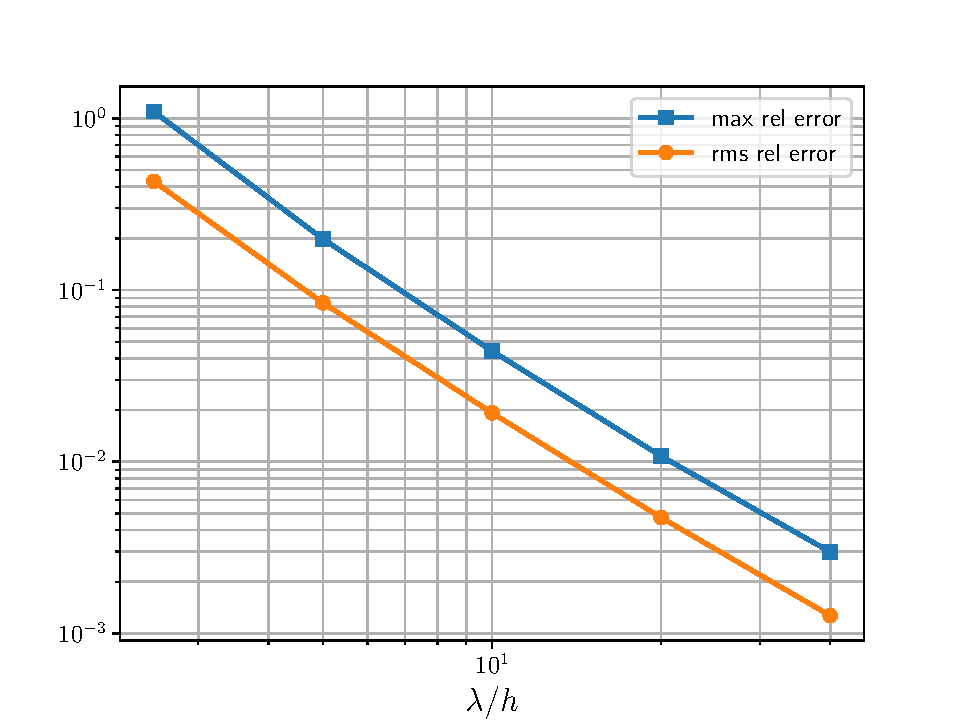
\includegraphics[width=0.45\textwidth]{verification_0.5lambda_pec_theta} &
      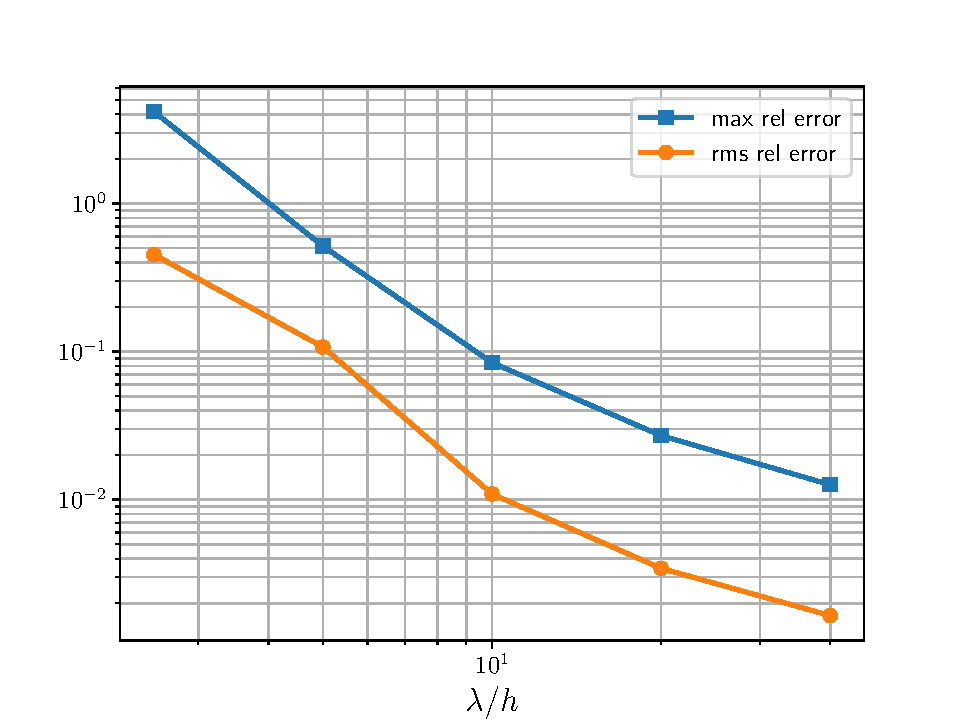
\includegraphics[width=0.45\textwidth]{verification_3.0lambda_pec_theta} \\
      (a) & (b) \\
      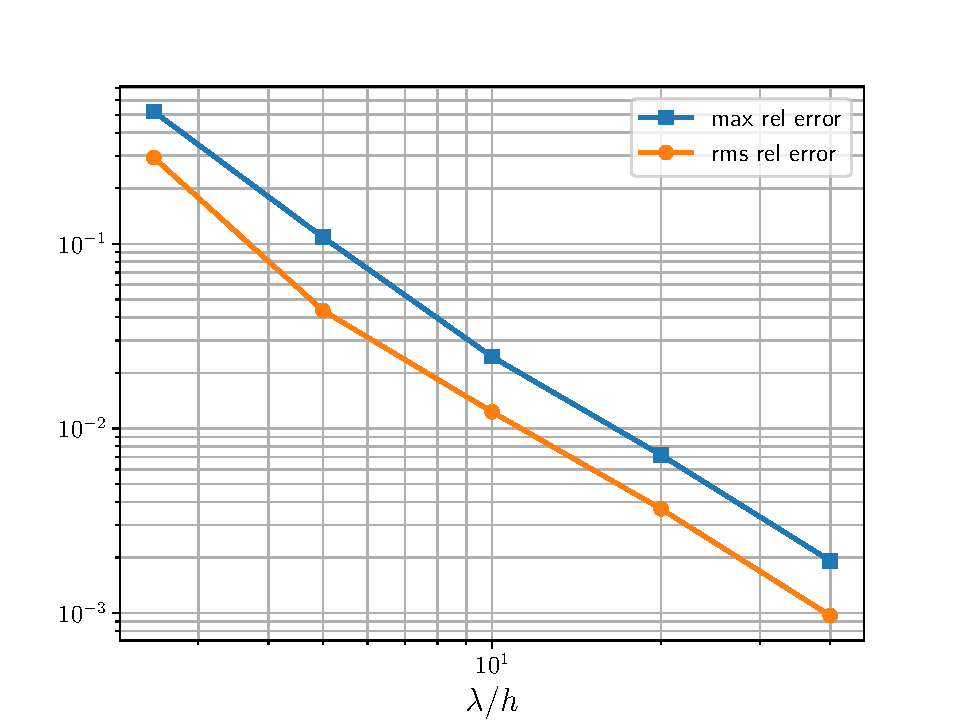
\includegraphics[width=0.45\textwidth]{verification_0.5lambda_dielectric_theta} &
      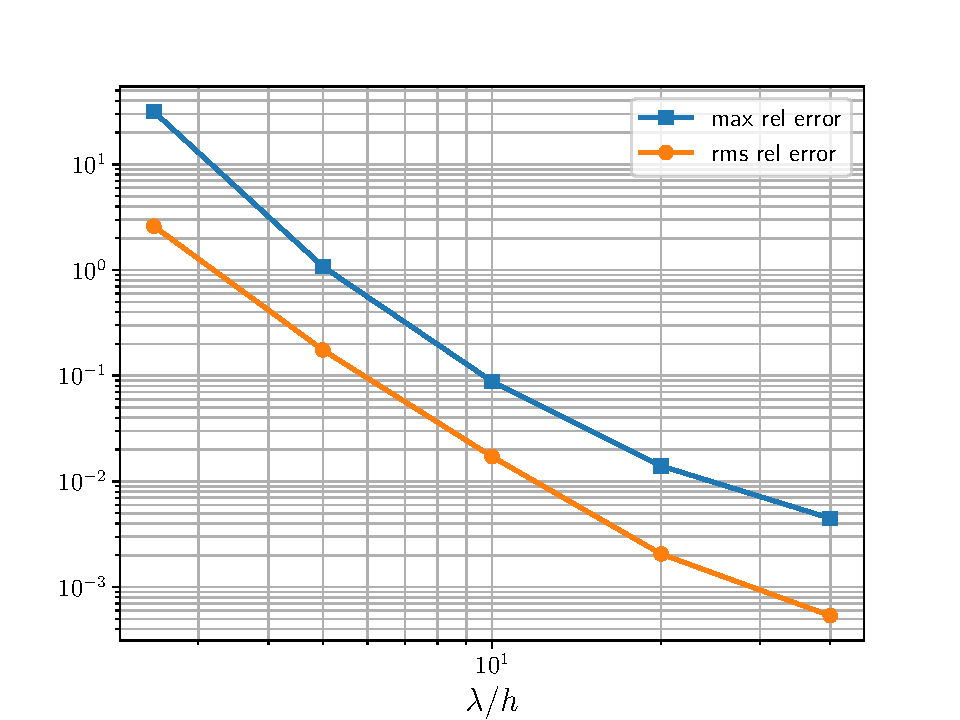
\includegraphics[width=0.45\textwidth]{verification_3.0lambda_dielectric_theta} \\
      (c) & (d) 
    \end{tabular}
  \end{center}
  \caption{Results for $h$-convergence of $E$-plane differential
    scattering cross section of some spheres. (a) PEC sphere radius
    $\lambda/2$, (b) PEC sphere radius $3\lambda$, (c) lossy
    dielectric sphere radius $\lambda/2$, (d) lossy dielectric sphere
    radius $3\lambda$.}
  \label{fig:hconvergence_Eplane}
\end{figure}

\begin{figure}
  \begin{center}
    \begin{tabular}{cc}
      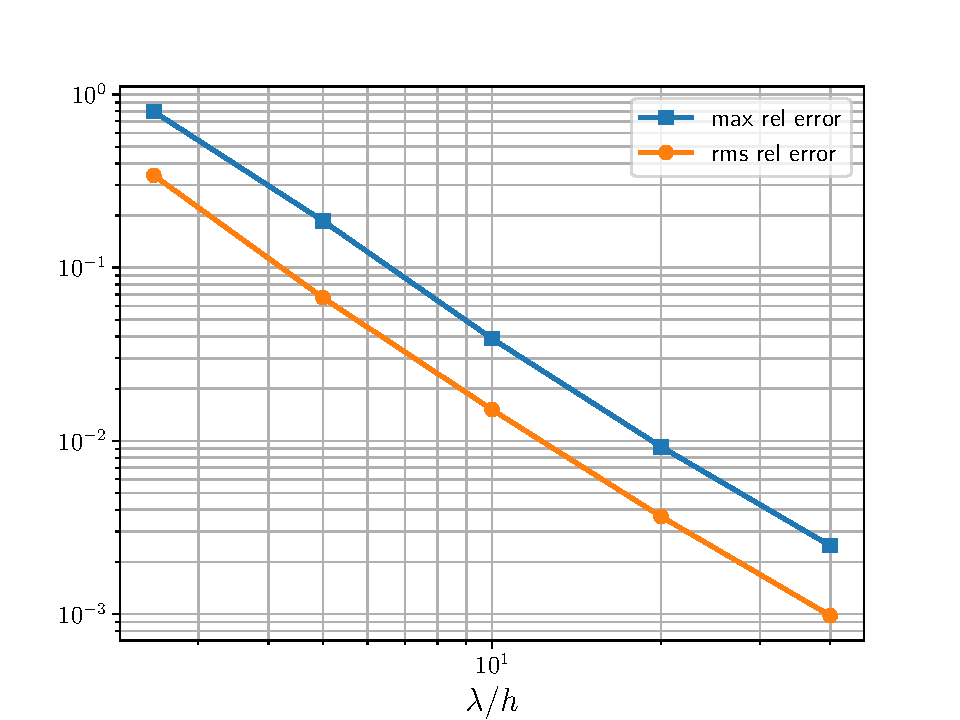
\includegraphics[width=0.45\textwidth]{verification_0.5lambda_pec_phi} &
      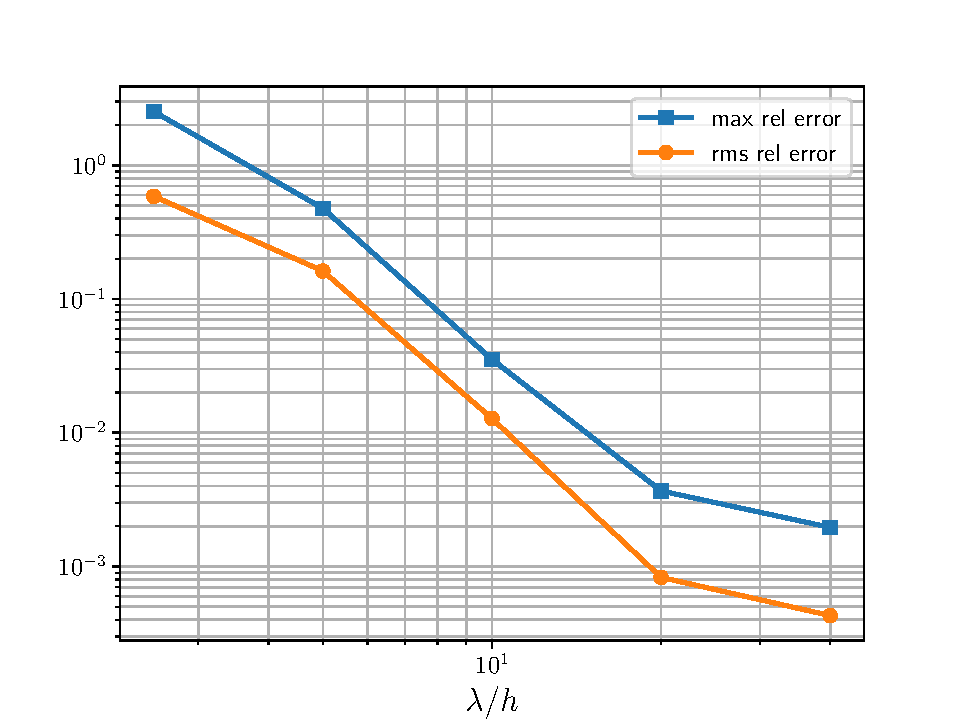
\includegraphics[width=0.45\textwidth]{verification_3.0lambda_pec_phi} \\
      (a) & (b) \\
      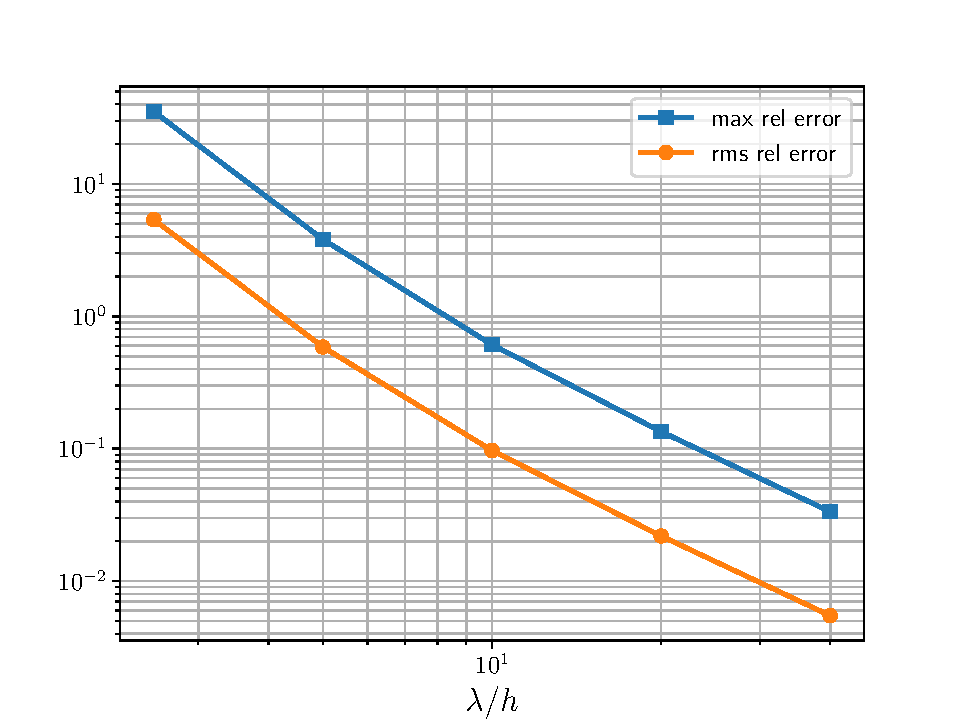
\includegraphics[width=0.45\textwidth]{verification_0.5lambda_dielectric_phi} &
      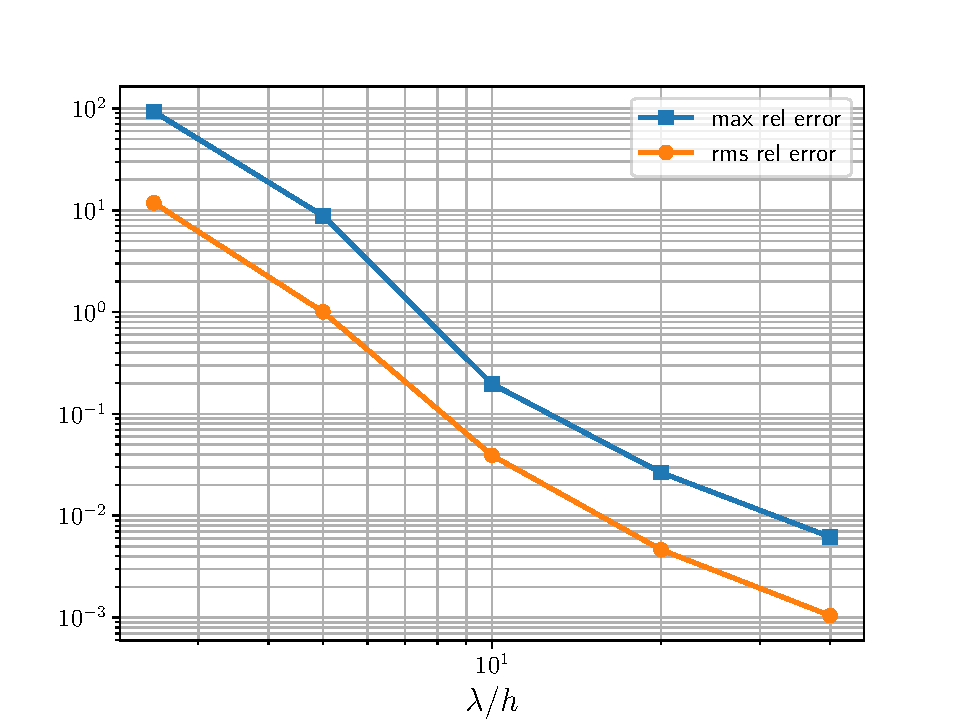
\includegraphics[width=0.45\textwidth]{verification_3.0lambda_dielectric_phi} \\
      (c) & (d) 
    \end{tabular}
  \end{center}
  \caption{Results for $h$-convergence of $H$-plane differential
    scattering cross section of some spheres. (a) PEC sphere radius
    $\lambda/2$, (b) PEC sphere radius $3\lambda$, (c) lossy
    dielectric sphere radius $\lambda/2$, (d) lossy dielectric sphere
    radius $3\lambda$.}
  \label{fig:hconvergence_Hplane}
\end{figure}

\section{Application to a radome geometry}

\begin{figure}
  \begin{center}
    \begin{tikzpicture}[>=latex]
      \pgfmathsetmacro{\ogivefactor}{2}
      \pgfmathsetmacro{\lda}{0.5}
      \pgfmathsetmacro{\w}{10*\lda}
      \pgfmathsetmacro{\H}{5*\lda}
      \pgfmathsetmacro{\epsr}{3}
      \pgfmathsetmacro{\d}{\lda/2/sqrt(\epsr)}
      \pgfmathsetmacro{\da}{\lda/2}
      \pgfmathsetmacro{\Rb}{\w/2 + \da + \d}
      \pgfmathsetmacro{\Lb}{\Rb*\ogivefactor}
      \pgfmathsetmacro{\rb}{(\Rb^2 + \Lb^2)/(2*\Rb)}
      \pgfmathsetmacro{\Ra}{\Rb - \d}
      \pgfmathsetmacro{\ra}{\rb - \d}
      \pgfmathsetmacro{\La}{sqrt(\ra^2 - (\rb - \Rb)^2)}
      \draw[smooth, samples=100, domain=0:1.0001] plot({sqrt(\ra^2-(\La*\x)^2) + \Ra - \ra}, \La*\x);
      \draw[smooth, samples=100, domain=0:1.0001] plot({sqrt(\rb^2-(\Lb*\x)^2) + \Rb - \rb}, \Lb*\x);
      \draw[smooth, samples=100, domain=0:1.001] plot({-(sqrt(\ra^2-(\La*\x)^2) + \Ra - \ra)}, \La*\x);
      \draw[smooth, samples=100, domain=0:1.001] plot({-(sqrt(\rb^2-(\Lb*\x)^2) + \Rb - \rb)}, \Lb*\x);
      \draw (\Ra,0) -- (\Ra,-\H) -- (\Rb,-\H) -- (\Rb,0);
      \draw (-\Ra,0) -- (-\Ra,-\H) -- (-\Rb,-\H) -- (-\Rb,0);
      \draw[ultra thick] (-\w/2,0) -- (\w/2,0);

      \draw[<->, shift={(0,-0.4)}] (-\w/2,0) -- (\w/2,0) node[midway, below] {$w$};
      \draw[<->, shift={(0,-1.4)}] (-\Ra,0) -- (\Ra,0) node[midway, below] {$2R_{\mrm{a}}$};
      \draw[<->, shift={(0,-2.4)}] (-\Rb,0) -- (\Rb,0) node[midway, below] {$2R_{\mrm{b}}$};
      \draw[<->, shift={(-0.5,0)}] (-\Rb,0) -- (-\Rb,-\H) node[midway,left] {$H$};
      \draw[<->] (0,0) -- (0,\La) node[midway, right] {$L_{\mrm{a}}$};
      \draw[<->, shift={(-\Rb-0.5,0)}] (0,0) -- (0,\Lb) node[midway, left] {$L_{\mrm{b}}$};
      \draw[dashed] (-\Rb-1,\Lb) -- (0.5,\Lb);
      \draw[->] (\Ra-0.5,-1) -- (\Ra,-1);
      \draw[->] (\Rb+1,-1) -- (\Rb,-1) node[midway,above] {$d$};
      \draw[->] (3,4) node[right] {$x=\sqrt{\rho_{\mrm{b}}^{2}-z^{2}} + R_{\mrm{b}} - \rho_{\mrm{b}}$} -- ({sqrt(\rb^2-(0.6*\Lb)^2)+\Rb-\rb},0.6*\Lb);
      \draw[->] (3,2) node[right] {$x=\sqrt{\rho_{\mrm{a}}^{2}-z^{2}} + R_{\mrm{a}} - \rho_{\mrm{a}}$} -- ({sqrt(\ra^2-(0.3*\La)^2)+\Ra-\ra},0.3*\La);
      \draw[->] (\Rb+0.5,0) -- (\Rb+1.5,0) node[right] {$x$};
      \draw[->] (0,\Lb+0.5) -- (0,\Lb+1.5) node[above] {$z$};
    \end{tikzpicture}
  \end{center}
  \caption{Geometry parameters of the ogive radome, adapted from
    \url{https://en.wikipedia.org/wiki/Nose_cone_design}. The radius
    of curvature for the ogive parts is computed from the other
    parameters as
    $\rho_{\mrm{a,b}} = (R_{\mrm{a,b}}^{2} +
    L_{\mrm{a,b}}^{2})/(2R_{\mrm{a,b}})$, and the thickness of the
    radome at the base is $d = R_{\mrm{b}} - R_{\mrm{a}}$. The antenna
    width is $w$, and the distance between the antenna and the radome
    is $d_{0} = R_{\mrm{a}} - w/2$.}
  \label{fig:ogiveradome_geometry}
\end{figure}

We analyze an ogive-shaped radome, which is a common design for a nose
cone radome, see Figure~\ref{fig:ogiveradome_geometry}. This design
has several features of a realistic radome, in particular a pointed
tip. The baseline parameters of the radome, corresponding to
Figure~\ref{fig:ogiveradome_geometry}, are chosen as
\begin{itemize}
\item $f_{0} = 10\unit{GHz}$ (frequency)
\item $\lambda_{0} = \cu/f_{0}$ (wavelength)
\item $w = 10\lambda_{0} = 0.300\unit{m}$ (diameter of antenna)
\item $d_{0} = \lambda_{0}/2 = 0.0150\unit{m}$ (distance from antenna to radome)
\item $\epsilon_{\mrm{r}} = 3$ (relative permittivity of radome, lossless)
\item $d = \lambda_{0}/(2\sqrt{\epsilon_{\mrm{r}}}) = 8.7\unit{mm}$
  (thickness of radome)
\item $\alpha = 2$ (ogive shape factor)
\item $R_{\mrm{a}} = w/2 + d_{0} = 0.165\unit{m}$
\item $L_{\mrm{a}} = \alpha R_{\mrm{a}} = 0.330\unit{m}$
\item $\rho_{\mrm{a}} = (R_{\mrm{a}}^{2} + L_{\mrm{a}}^{2})/(2R_{\mrm{a}}) = 0.412\unit{m}$
\item $R_{\mrm{b}} = w/2 + d_{0} + d = 0.174\unit{m}$
\item $L_{\mrm{b}} = \alpha R_{\mrm{b}} = 0.347\unit{m}$
\item $\rho_{\mrm{b}} = (R_{\mrm{b}}^{2} + L_{\mrm{b}}^{2})/(2R_{\mrm{b}}) = 0.434\unit{m}$
\item $H = 5\lambda_{0} = 0.150\unit{m}$
\end{itemize}
The antenna is implemented as a circular antenna with thickness
$0.1\lambda_{0}$ and a cosine-tapering in the radial direction, that
is, the antenna field is
\begin{equation}
  \Ev_{\mrm{a}}(\rv) = \Ev_{0}\eu^{-\ju\kv\cdot\rv}\cos(\pi\rho/w), \quad \rv\in\Gamma_{\mrm{ant}}
\end{equation}
where the expression for a plane wave in \eqref{eq:planewave} is used
to express $\Ev_{0}\eu^{-\ju\kv\cdot\rv}$ in azimuthal modes. The
baseline antenna is ten wavelengths in diameter, making the radiation
highly directive.


\subsection{Parameter variations}

From the baseline geometry we make a number of parameter variations in
the simulations:
\begin{itemize}
\item Electric field in $\theta$ (TM, in plane) or $\phi$ (TE, out of
  plane) polarization.
\item Angle of incidence $\theta\in[0^{\circ},10^{\circ},20^{\circ},30^{\circ},40^{\circ},50^{\circ}]$.
\item With and without radome.
\item Either with a transmitting antenna or scattering from an
  incident plane wave.
\item Antenna width
  $w\in[10\lambda_{0},20\lambda_{0},30\lambda_{0}]$. Note that the
  radome thickness is $\lambda_{0}/(2\sqrt{\epsilon_{\mrm{r}}})$ in
  all cases, that is, the radome is always transparent.
\end{itemize}
All combinations of these parameters are run, except for
$w=30\lambda_{0}$ where the angles are reduced to
$\theta\in[0^{\circ},30^{\circ},50^{\circ}]$ (this simulation took
about as long as all the others together, a bit more than one week on
an ordinary desktop computer).

\subsection{Results}

\newlength{\myfigwidth}
\setlength{\myfigwidth}{0.5\linewidth}

\begin{figure}
  \begin{center}
    \begin{tabular}{ccc}
      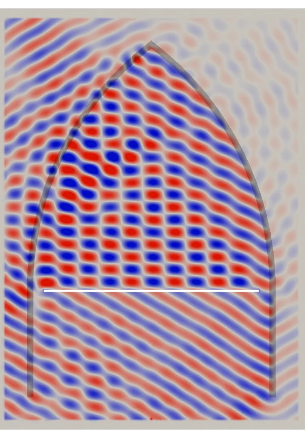
\includegraphics[width=0.3\linewidth]{nearfield_scattering_theta30_w10} &
      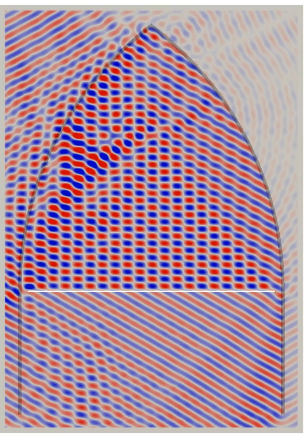
\includegraphics[width=0.3\linewidth]{nearfield_scattering_theta30_w20} &
      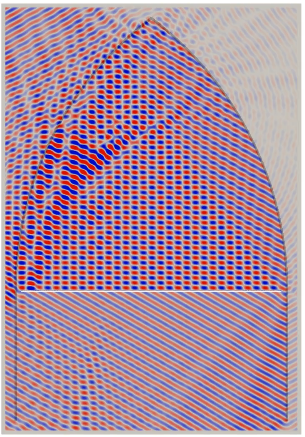
\includegraphics[width=0.3\linewidth]{nearfield_scattering_theta30_w30} \\
      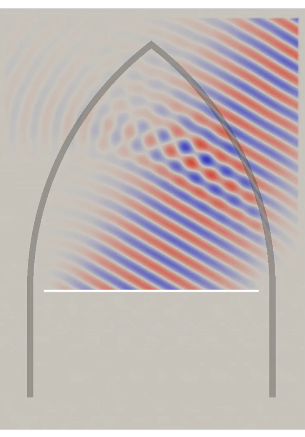
\includegraphics[width=0.3\linewidth]{nearfield_transmitting_theta30_w10} &
      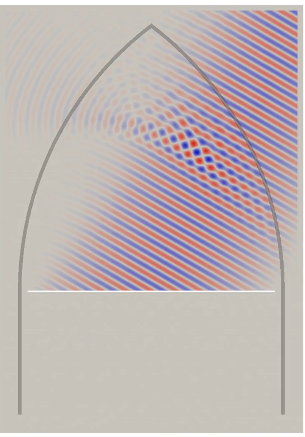
\includegraphics[width=0.3\linewidth]{nearfield_transmitting_theta30_w20} &
      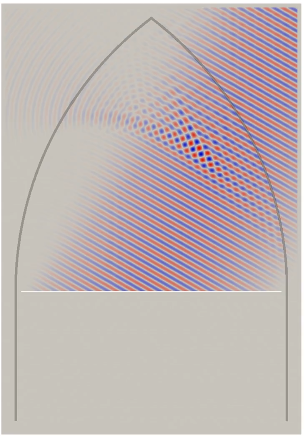
\includegraphics[width=0.3\linewidth]{nearfield_transmitting_theta30_w30} 
    \end{tabular}
  \end{center}
  \caption{Near field plots of scattered field when subjected to an
    incident plane wave from $\theta=30^{\circ}$ (top row) and total
    field with transmitting antenna towards $\theta=30^{\circ}$
    (bottom row) from antenna with and without radome, antenna widths
    $w=10\lambda_{0},20\lambda_{0},30\lambda_{0}$ (from left to
    right).}
  \label{fig:nearfields}
\end{figure}


\begin{figure}
  \begin{center}
    \begin{tabular}{cc}
      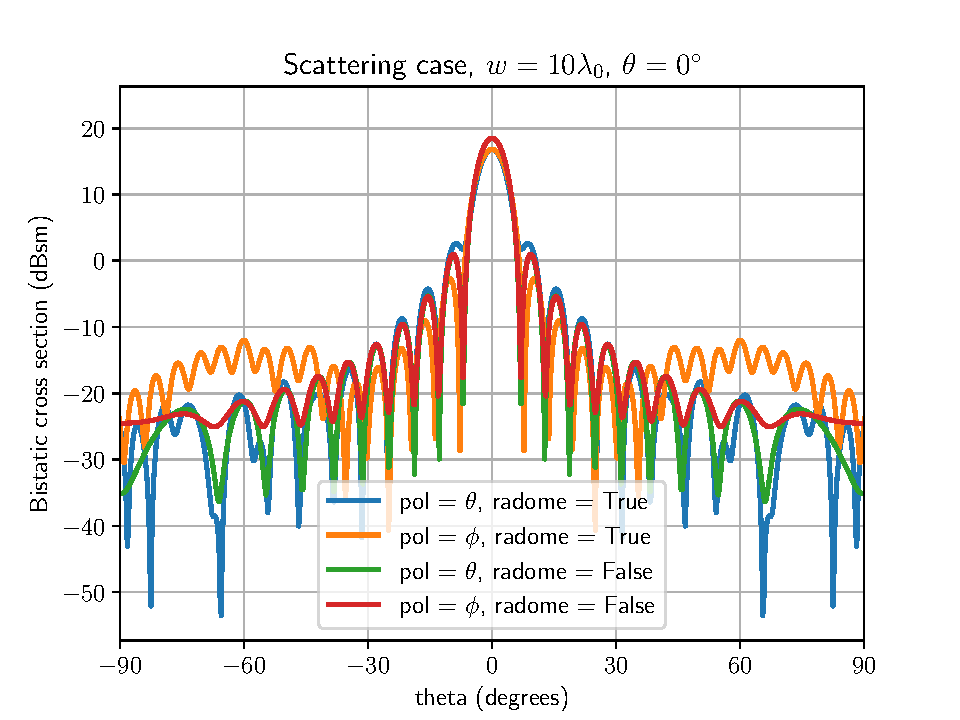
\includegraphics[width=\myfigwidth]{scattering_w10_theta0} &
      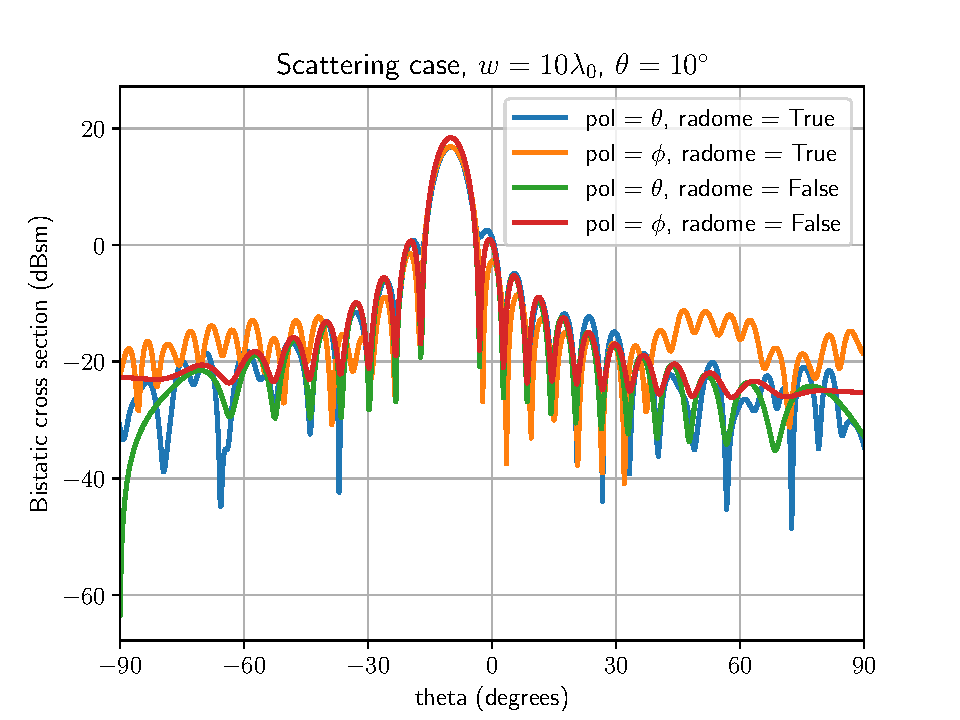
\includegraphics[width=\myfigwidth]{scattering_w10_theta10} \\
      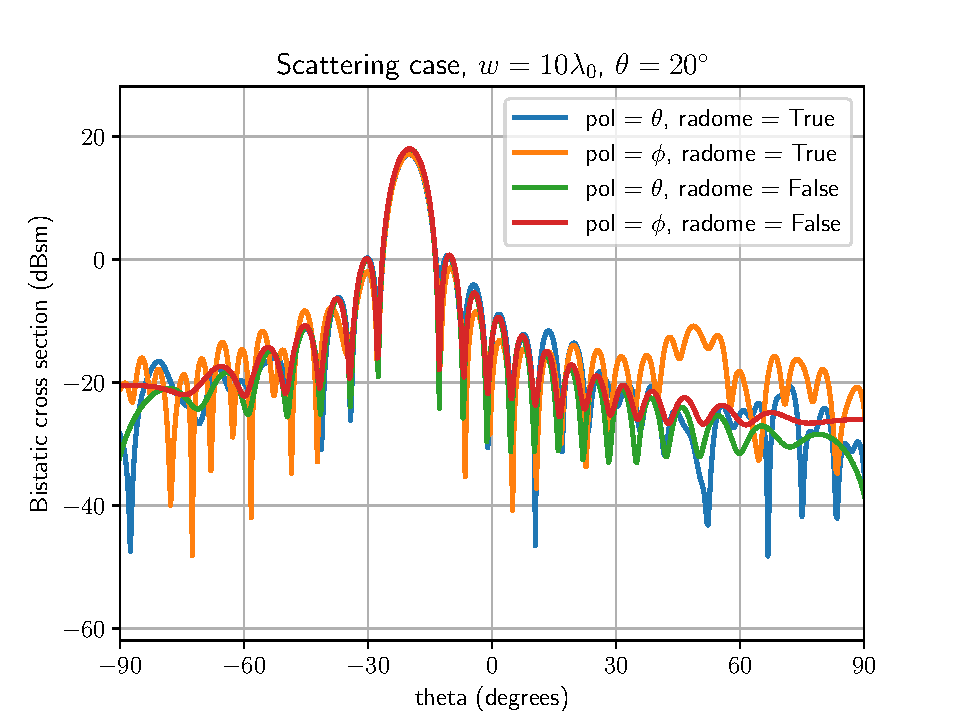
\includegraphics[width=\myfigwidth]{scattering_w10_theta20} &
      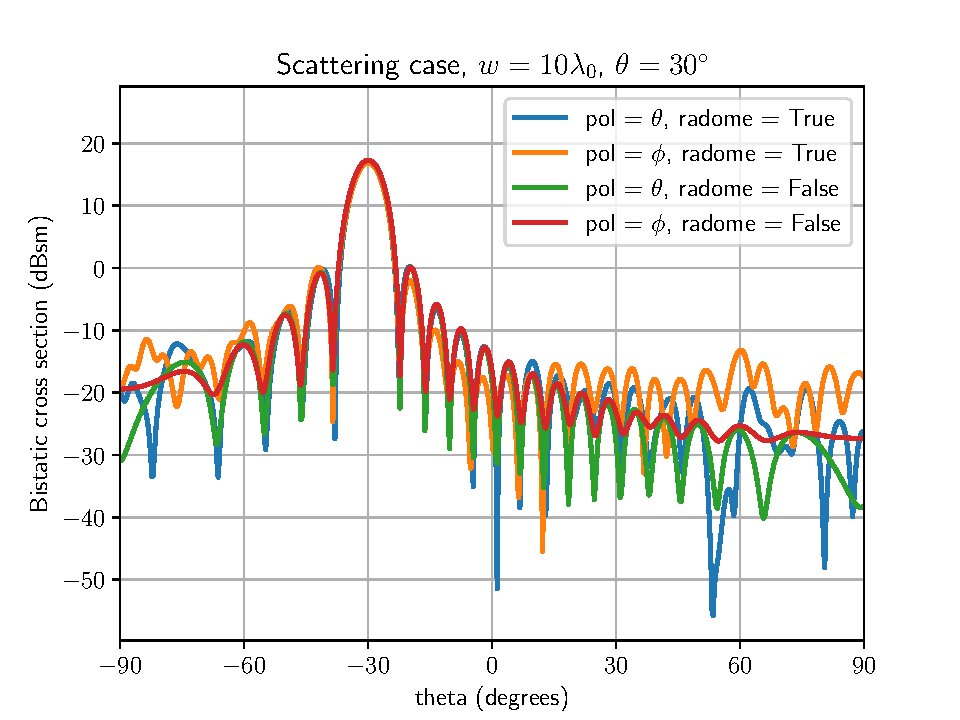
\includegraphics[width=\myfigwidth]{scattering_w10_theta30} \\
      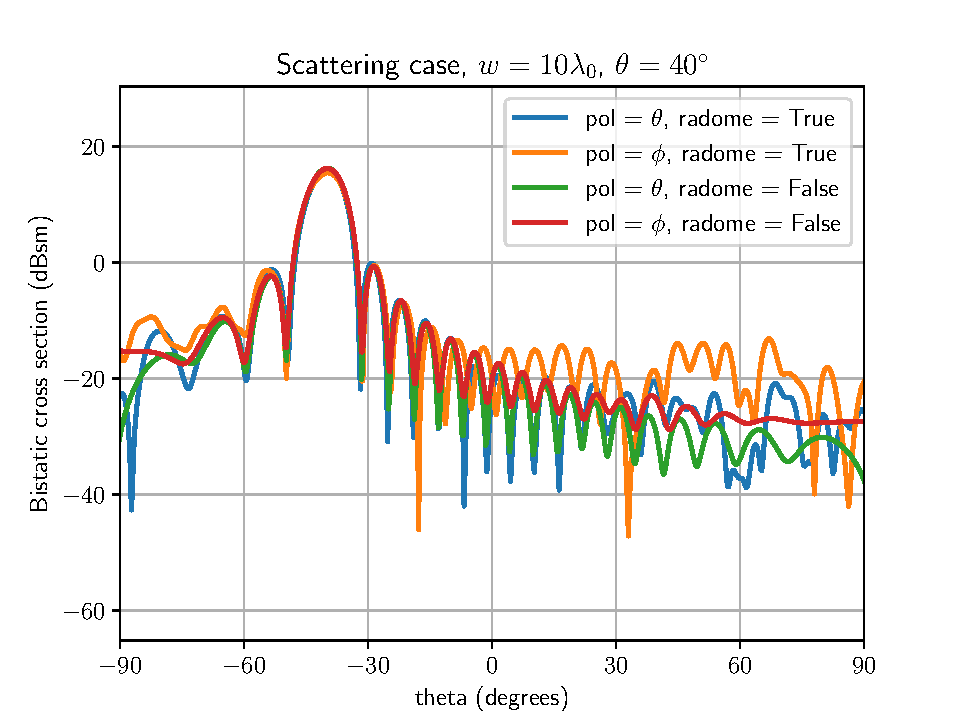
\includegraphics[width=\myfigwidth]{scattering_w10_theta40} &
      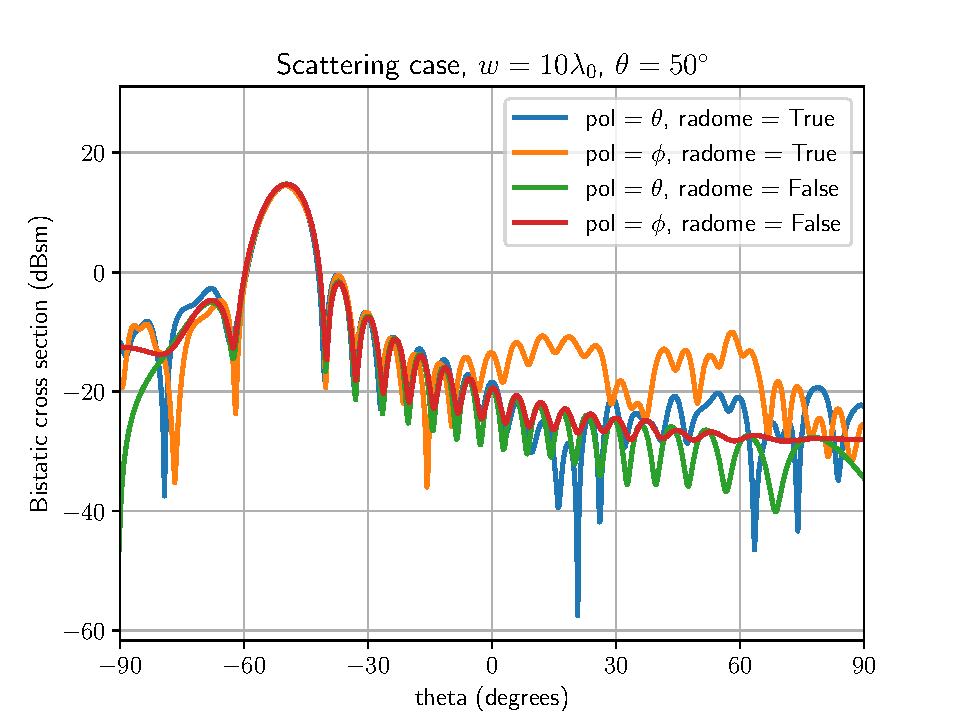
\includegraphics[width=\myfigwidth]{scattering_w10_theta50} 
    \end{tabular}
  \end{center}
  \caption{Scattering from antenna with and without radome, antenna
    width $w=10\lambda_{0}$.}
  \label{fig:scatteringw10}
\end{figure}

\begin{figure}
  \begin{center}
    \begin{tabular}{cc}
      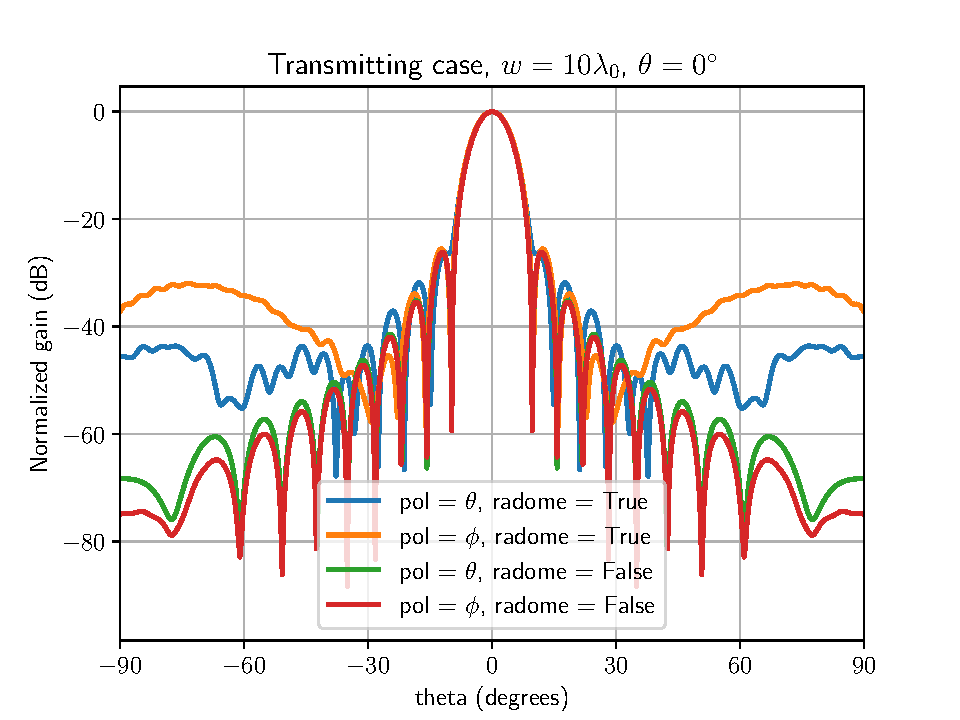
\includegraphics[width=\myfigwidth]{transmitting_w10_theta0} &
      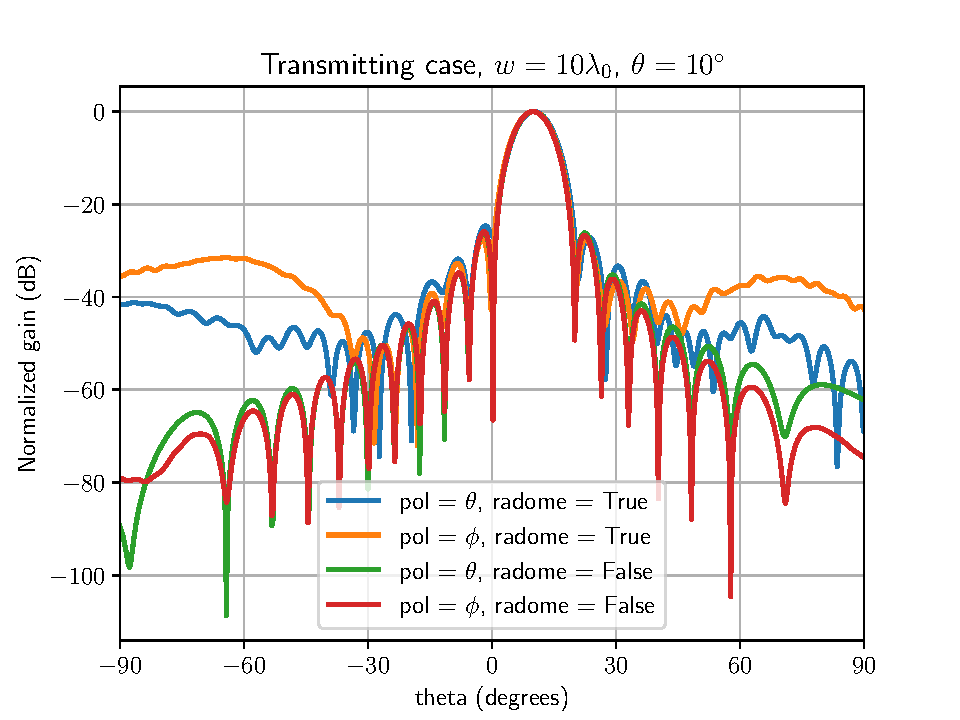
\includegraphics[width=\myfigwidth]{transmitting_w10_theta10} \\
      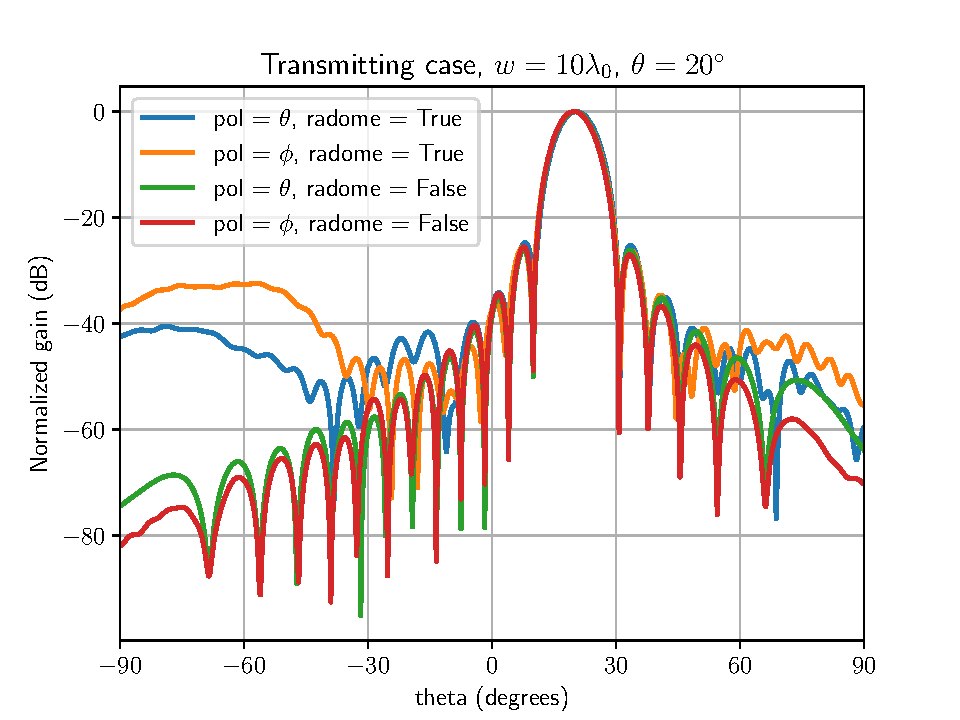
\includegraphics[width=\myfigwidth]{transmitting_w10_theta20} &
      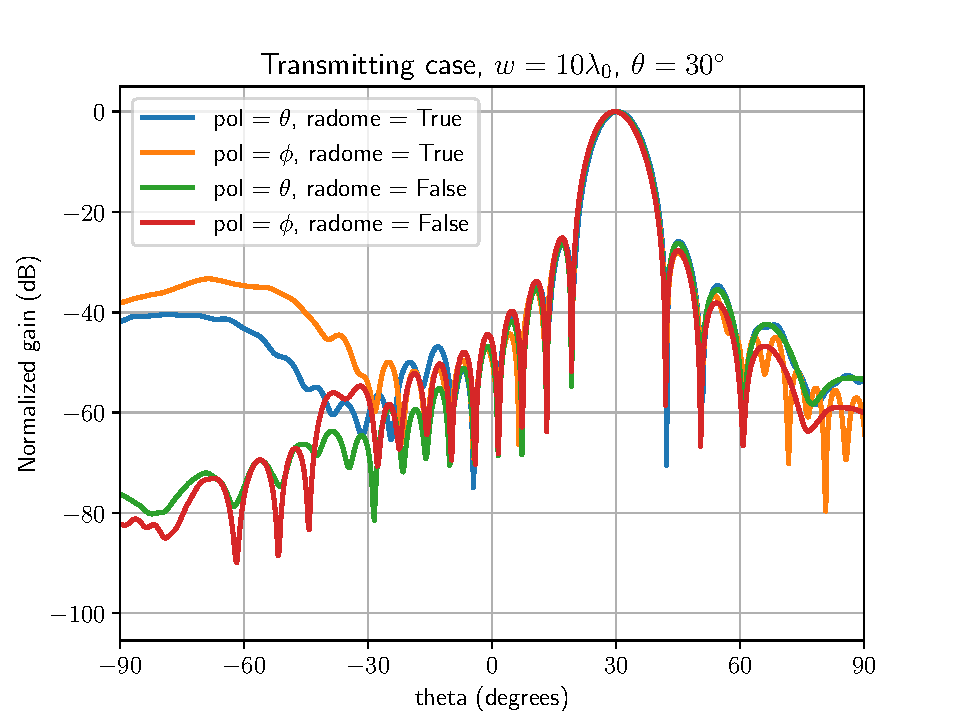
\includegraphics[width=\myfigwidth]{transmitting_w10_theta30} \\
      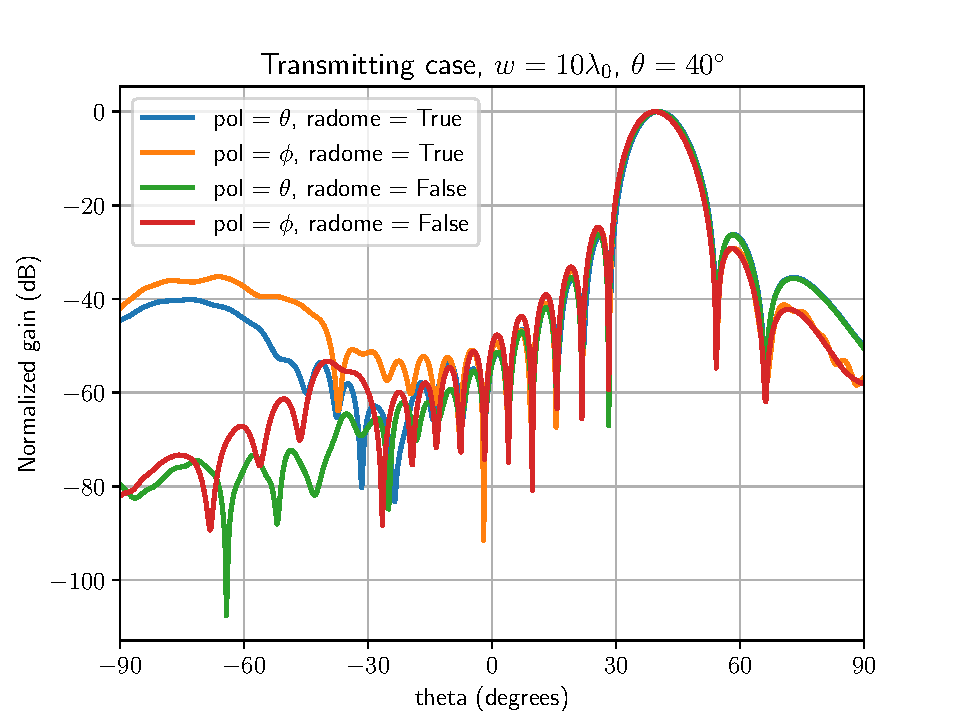
\includegraphics[width=\myfigwidth]{transmitting_w10_theta40} &
      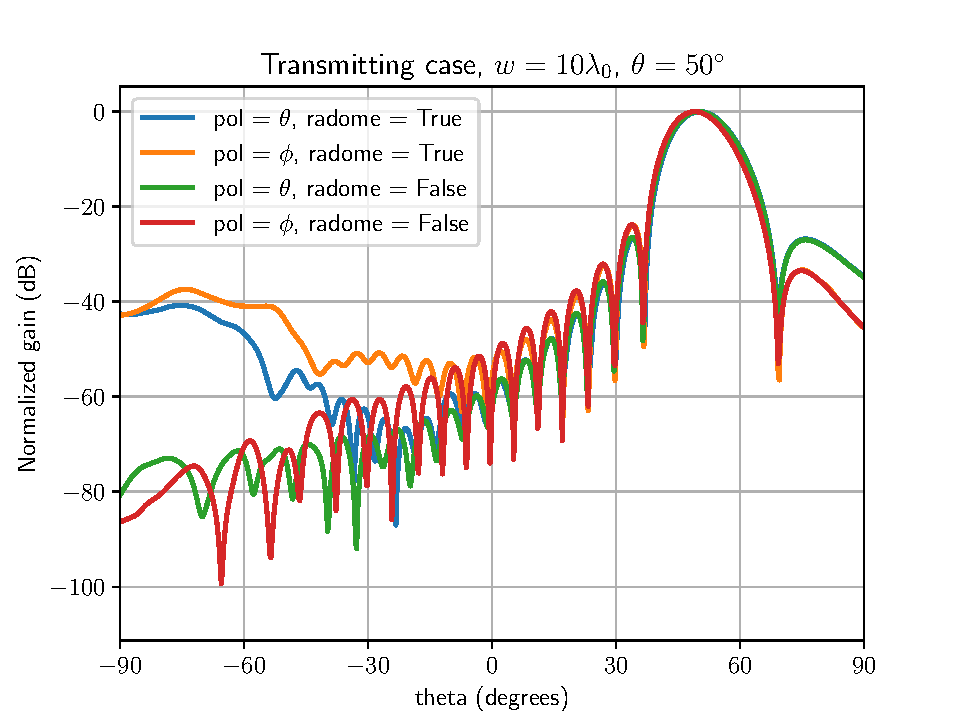
\includegraphics[width=\myfigwidth]{transmitting_w10_theta50} 
    \end{tabular}
  \end{center}
  \caption{Transmission from antenna with and without radome, antenna
    width $w=10\lambda_{0}$.}
  \label{fig:transmissionw10}
\end{figure}

\begin{figure}
  \begin{center}
    \begin{tabular}{cc}
      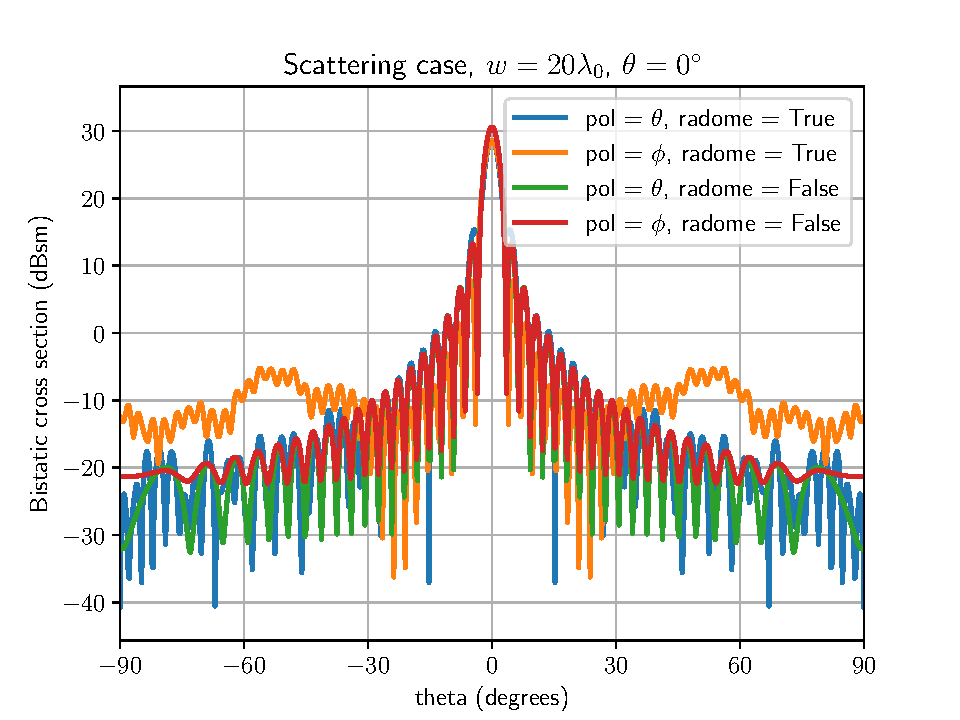
\includegraphics[width=\myfigwidth]{scattering_w20_theta0} &
      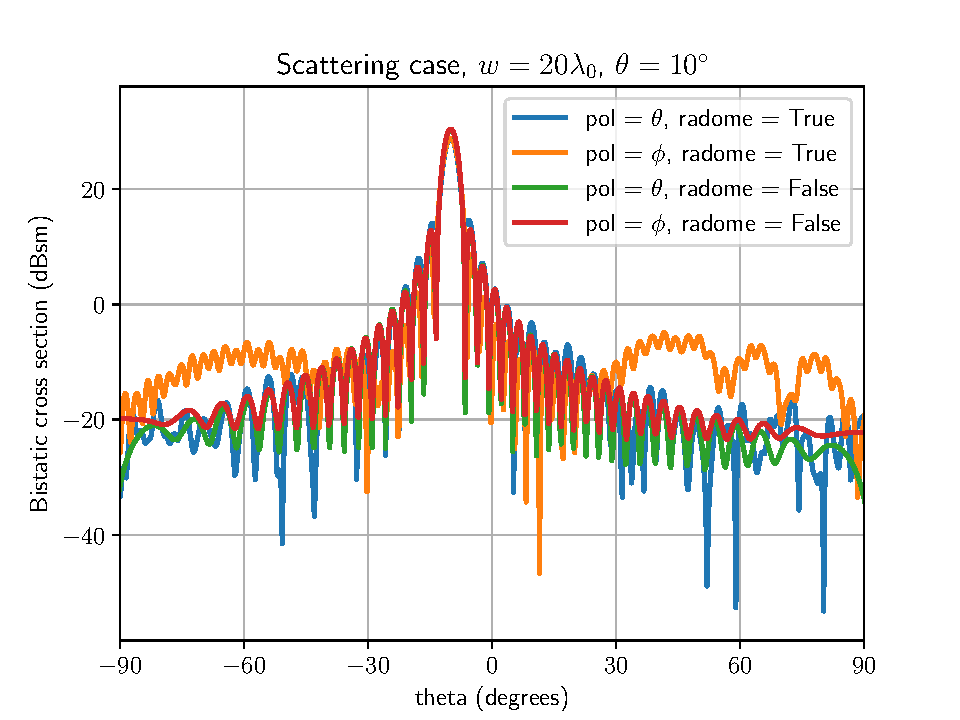
\includegraphics[width=\myfigwidth]{scattering_w20_theta10} \\
      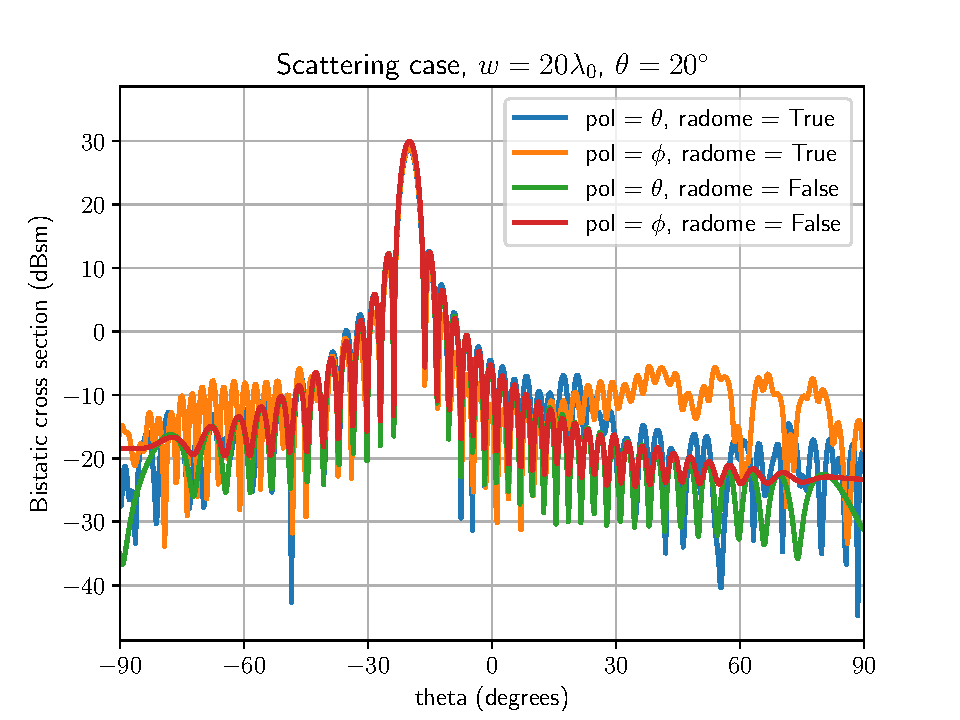
\includegraphics[width=\myfigwidth]{scattering_w20_theta20} &
      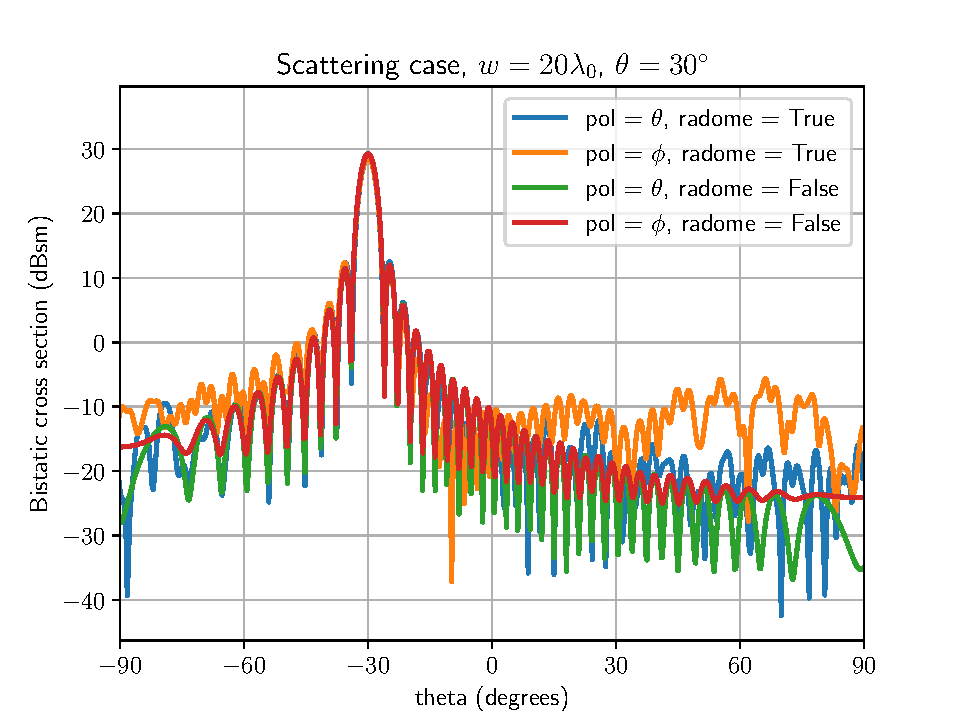
\includegraphics[width=\myfigwidth]{scattering_w20_theta30} \\
      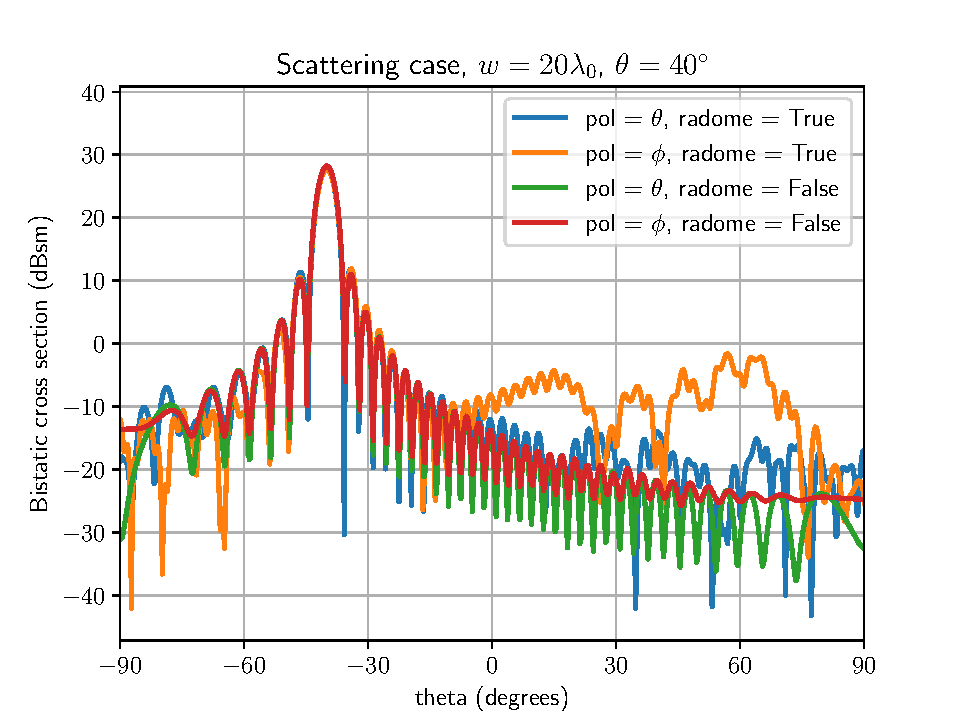
\includegraphics[width=\myfigwidth]{scattering_w20_theta40} &
      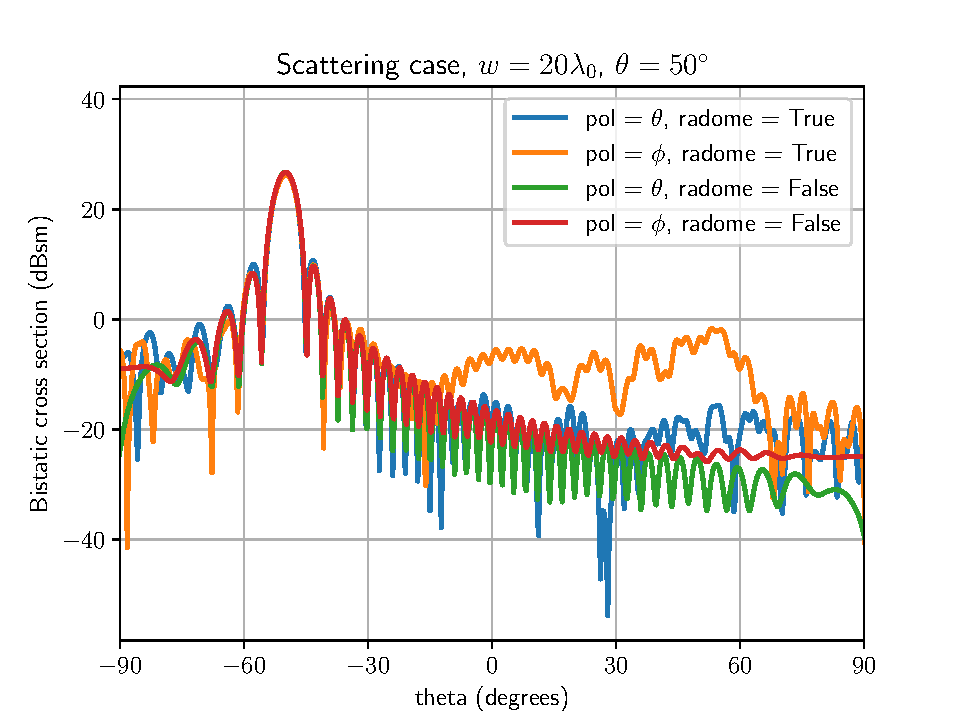
\includegraphics[width=\myfigwidth]{scattering_w20_theta50} 
    \end{tabular}
  \end{center}
  \caption{Scattering from antenna with and without radome, antenna
    width $w=20\lambda_{0}$.}
  \label{fig:scatteringw20}
\end{figure}

\begin{figure}
  \begin{center}
    \begin{tabular}{cc}
      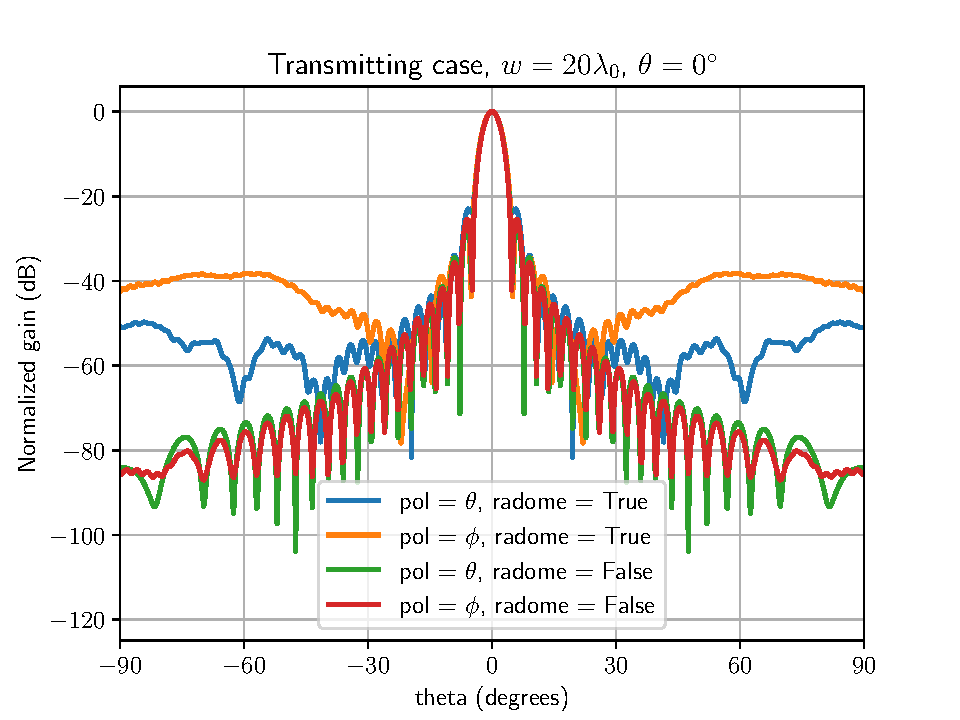
\includegraphics[width=\myfigwidth]{transmitting_w20_theta0} &
      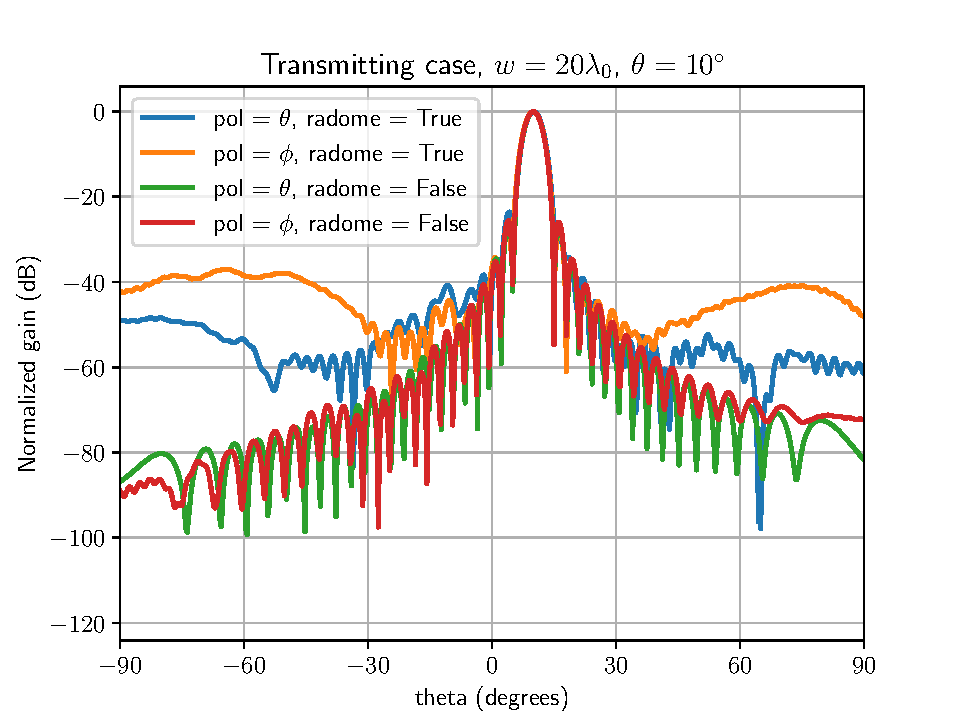
\includegraphics[width=\myfigwidth]{transmitting_w20_theta10} \\
      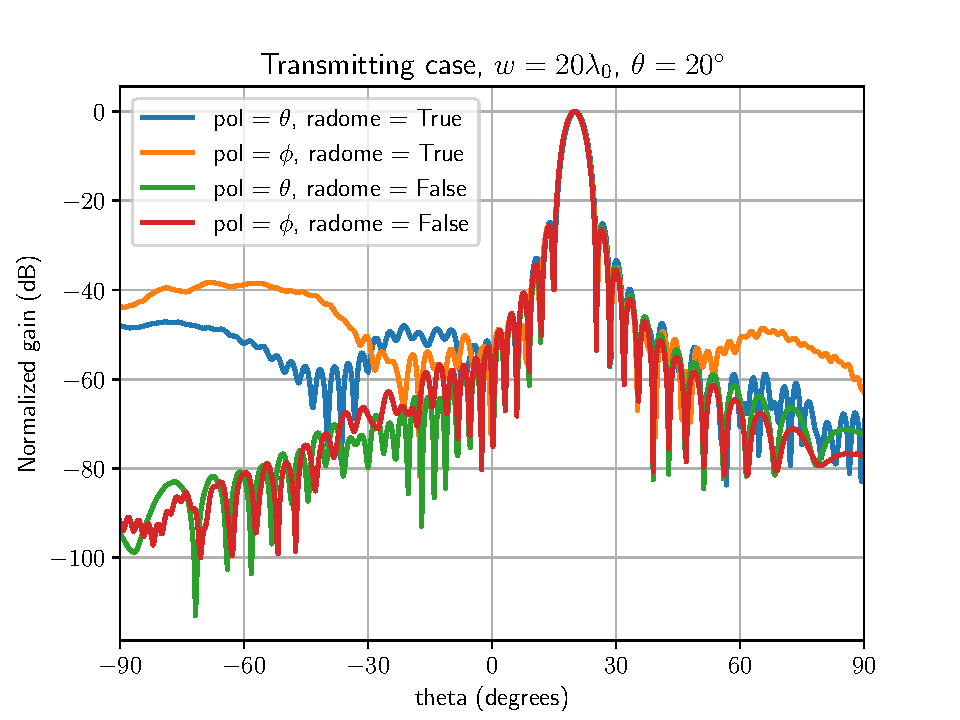
\includegraphics[width=\myfigwidth]{transmitting_w20_theta20} &
      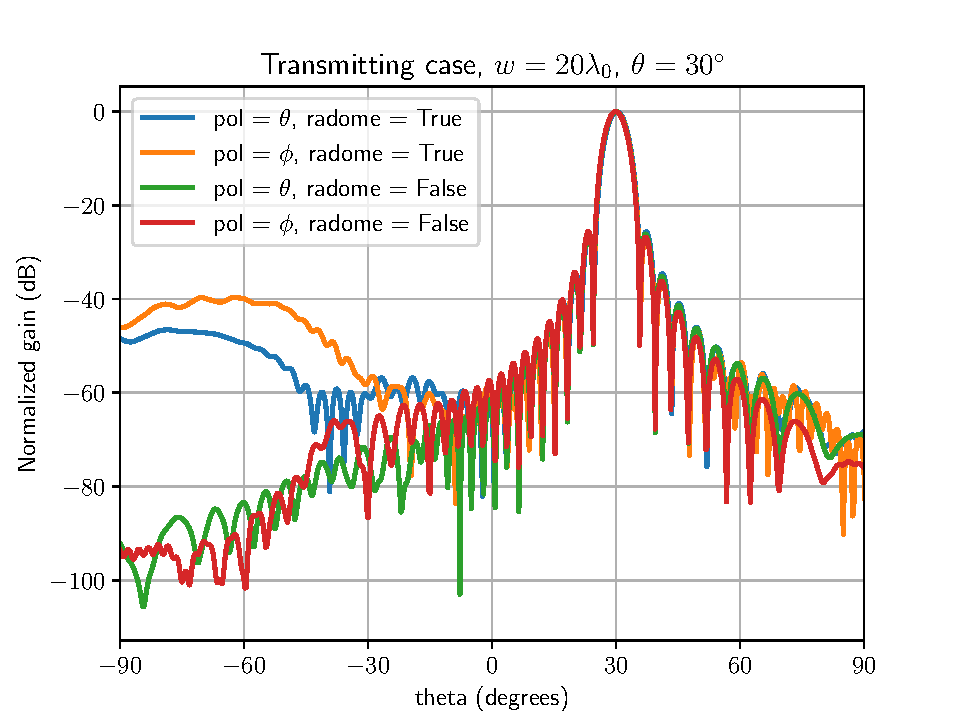
\includegraphics[width=\myfigwidth]{transmitting_w20_theta30} \\
      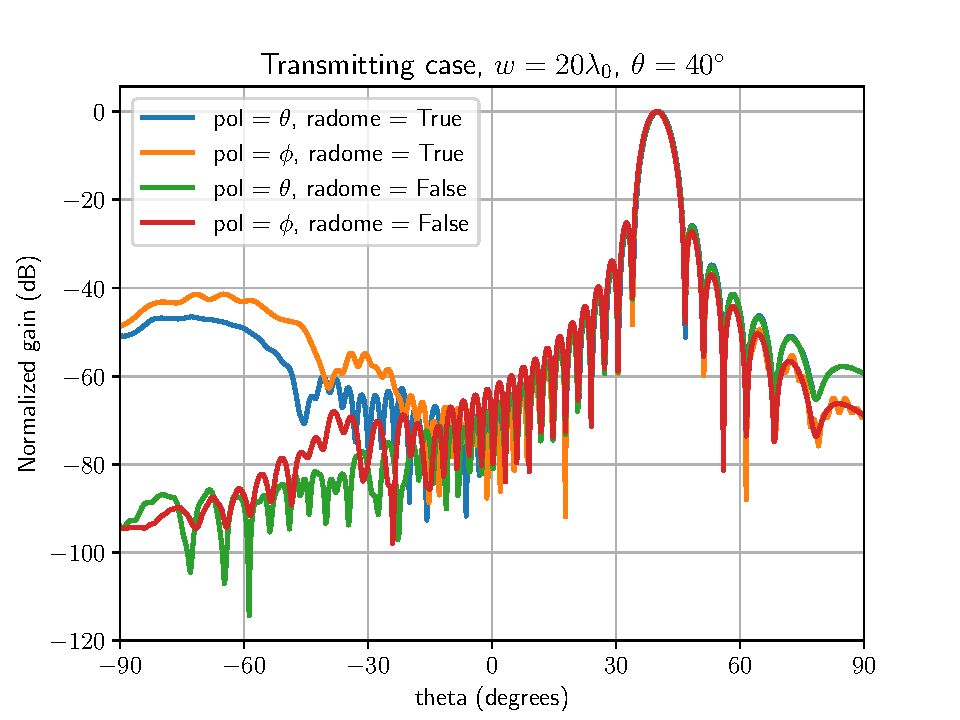
\includegraphics[width=\myfigwidth]{transmitting_w20_theta40} &
      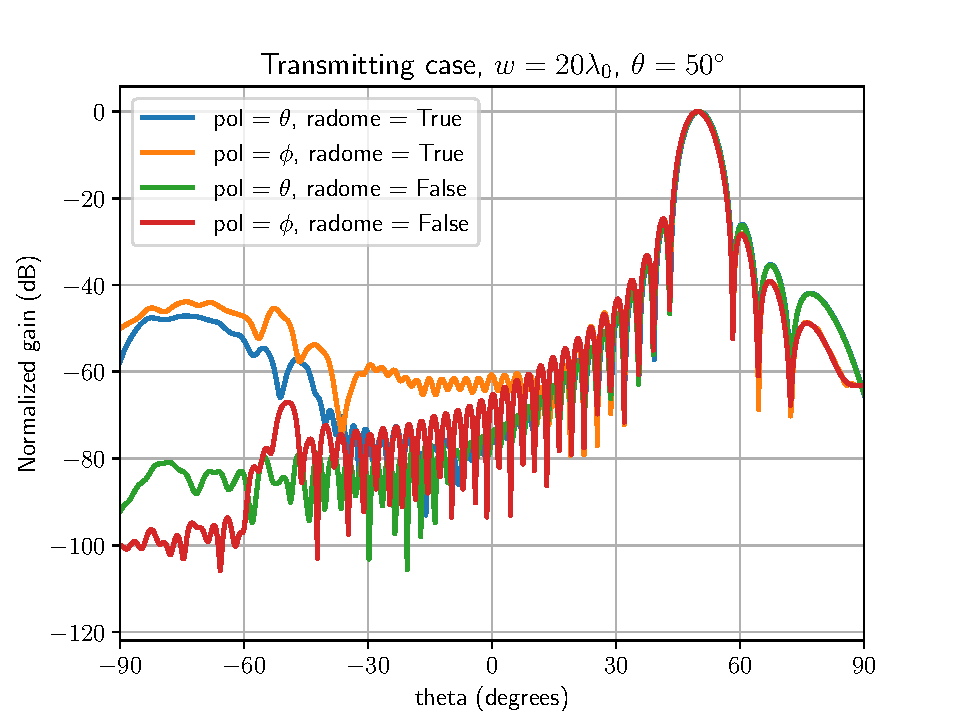
\includegraphics[width=\myfigwidth]{transmitting_w20_theta50} 
    \end{tabular}
  \end{center}
  \caption{Transmission from antenna with and without radome, antenna
    width $w=20\lambda_{0}$.}
  \label{fig:transmissionw20}
\end{figure}

\begin{figure}
  \begin{center}
    \begin{tabular}{cc}
      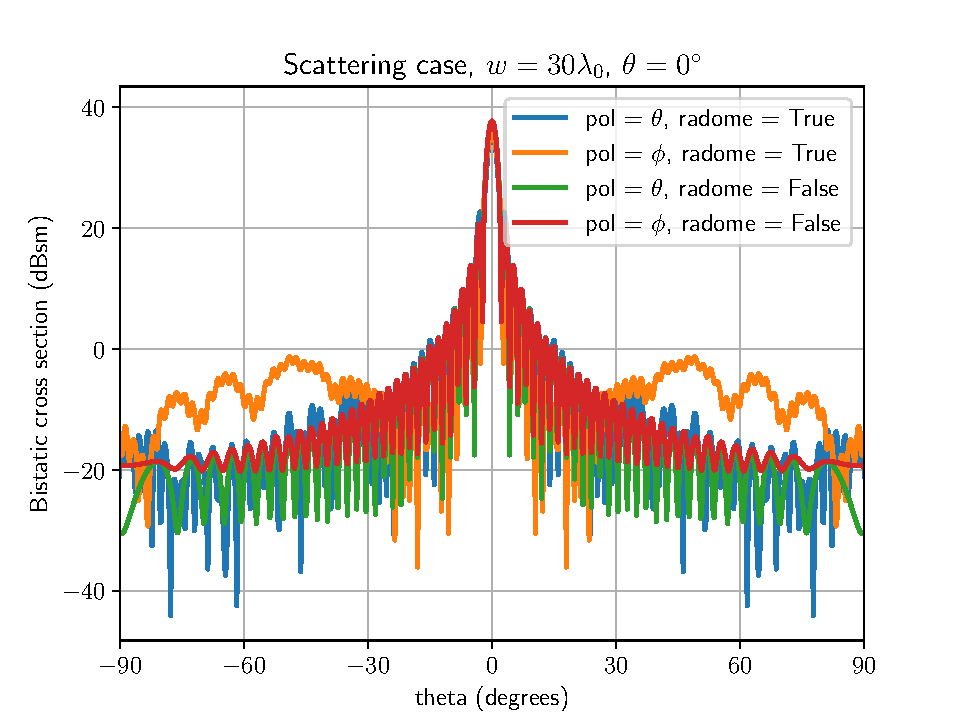
\includegraphics[width=\myfigwidth]{scattering_w30_theta0} &
      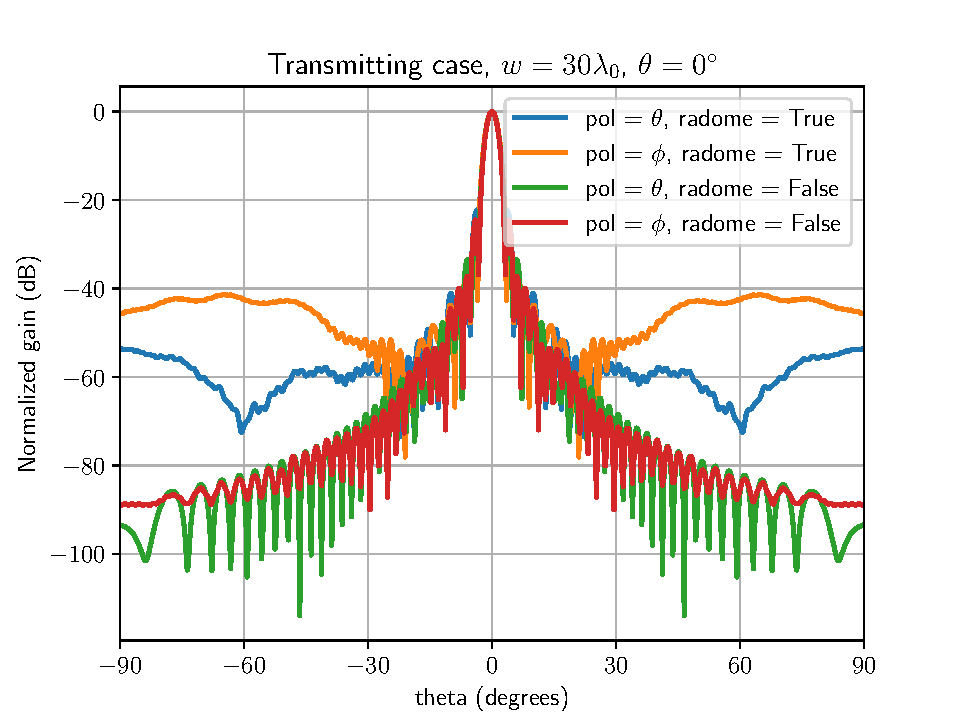
\includegraphics[width=\myfigwidth]{transmitting_w30_theta0} \\
      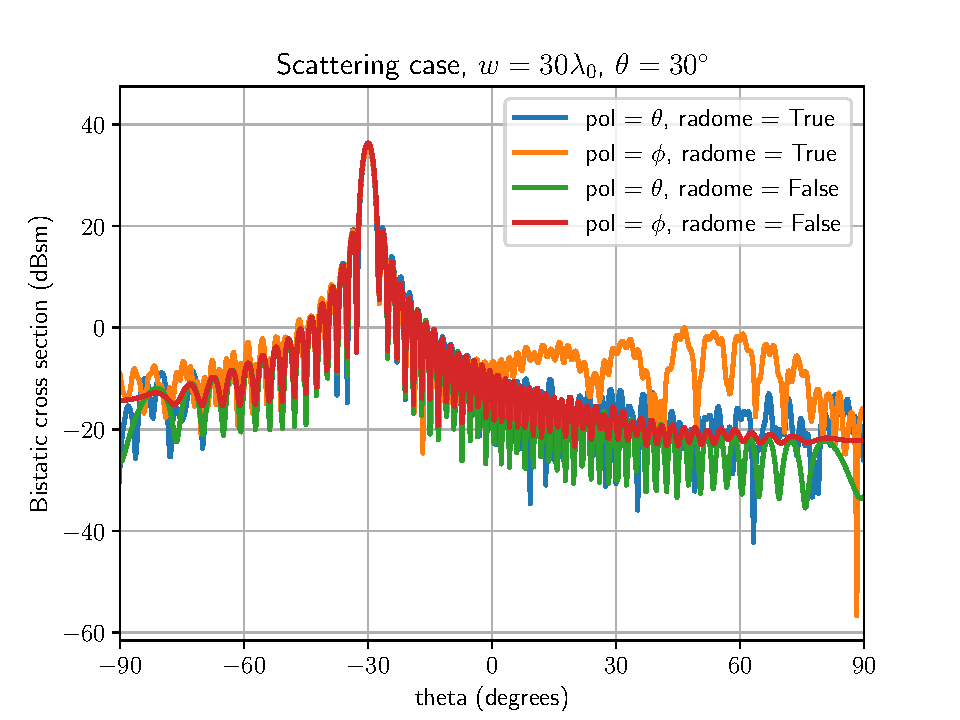
\includegraphics[width=\myfigwidth]{scattering_w30_theta30} &
      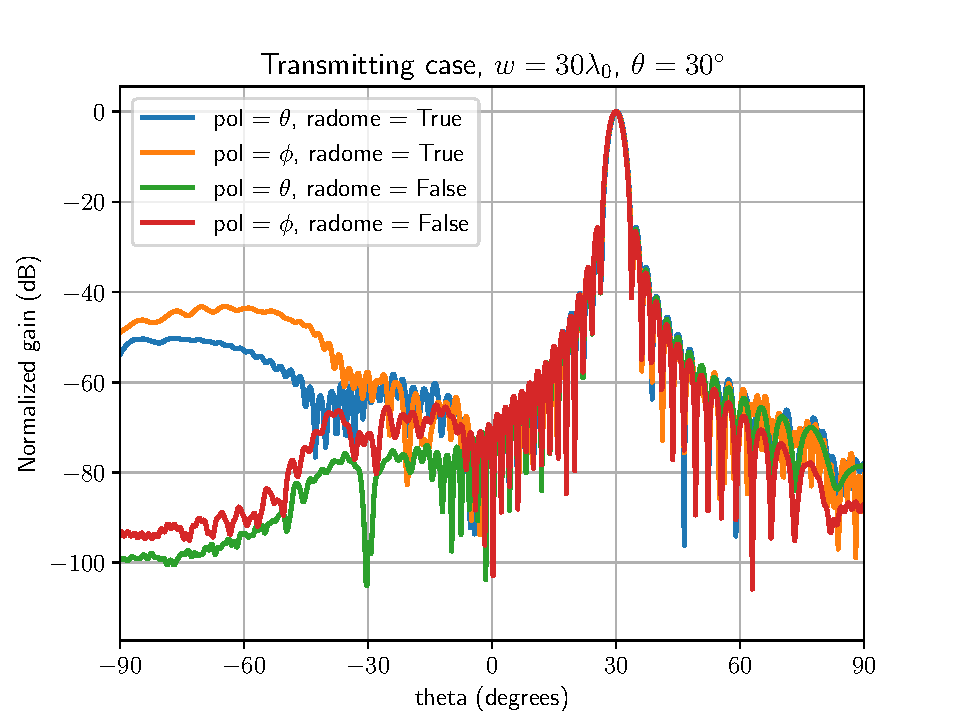
\includegraphics[width=\myfigwidth]{transmitting_w30_theta30} \\
      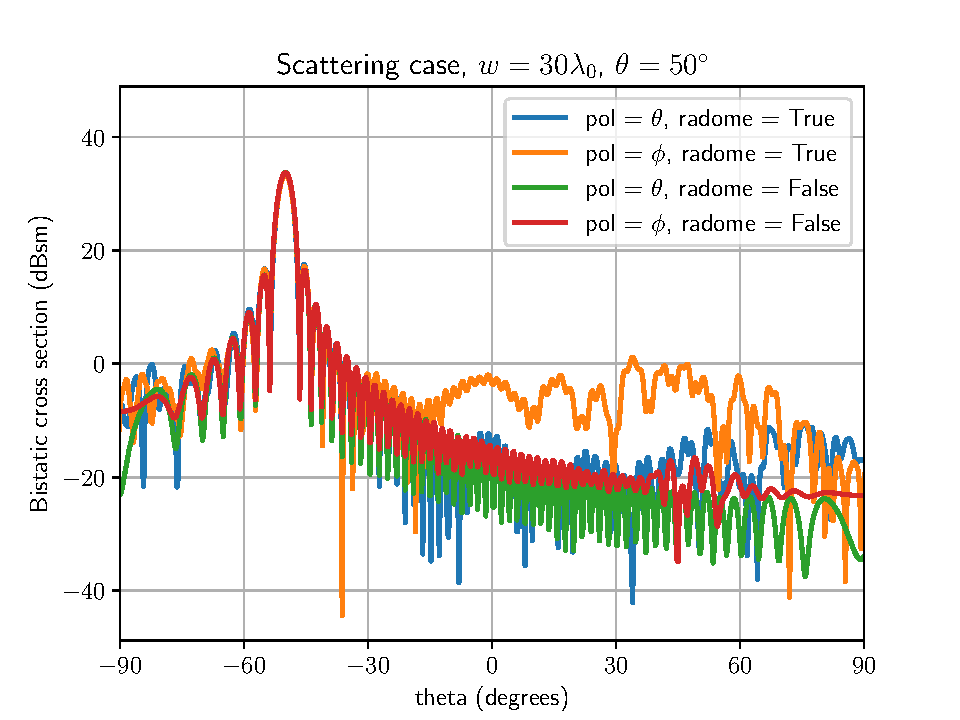
\includegraphics[width=\myfigwidth]{scattering_w30_theta50} &
      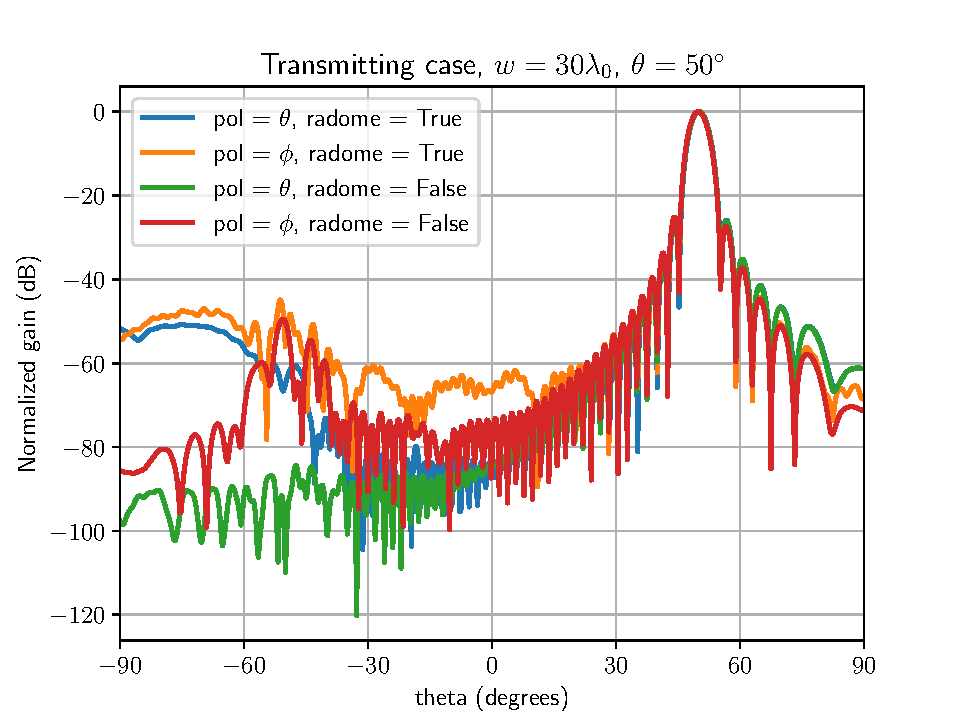
\includegraphics[width=\myfigwidth]{transmitting_w30_theta50} 
    \end{tabular}
  \end{center}
  \caption{Scattering (left column) and transmission (right column)
    from antenna with and without radome, antenna width
    $w=30\lambda_{0}$.}
  \label{fig:scatteringtransmissionw30}
\end{figure}


\section{Conclusions}
\label{sec:conclusions}



\newpage

\appendix

\section{Computation of far field amplitudes}
\label{app:farfield}

In this Appendix, we give explicit derivations of how the far field
amplitudes used in the computational examples can be derived. The
general setup of solving Maxwell's equations in a rotationally
symmetric geometry is provided in Section~\ref{sec:rotational}. There,
it is seen that the fields can be represented in cylindrical
coordinates $(\rho,\varphi,z)$ as
\begin{align}
  \Ev(\rv) &= \sum_{m=-\infty}^{\infty} \left[E_{\rho}^{(m)}(\rho,z)\rhouv + E_{\varphi}^{(m)}(\rho,z)\varphiuv + E_{z}^{(m)}(\rho,z)\zuv \right] \eu^{-\ju m\varphi} \\
  \Hv(\rv) &= \sum_{m=-\infty}^{\infty} \left[H_{\rho}^{(m)}(\rho,z)\rhouv + H_{\varphi}^{(m)}(\rho,z)\varphiuv + H_{z}^{(m)}(\rho,z)\zuv \right] \eu^{-\ju m\varphi}
\end{align}
In this Appendix, we demonstrate how to solve the azimuthal part of
the far field integral 
\begin{equation}
  \Fv(\kuv) = \frac{\ju k}{4\pi} \kuv\times \int_{S} \left[ \Ev(\rv)\times\nuv + \eta_{0}\kuv\times(\nuv\times\Hv(\rv)) \right] \eu^{\ju k\kuv\cdot\rv} \diff S
\end{equation}
for arbitrary azimuthal mode index $m$. The radiation direction $\kuv$
is parameterized by the standard polar angle $\theta$ and azimuth
angle $\phi$.

The fields $\Ev^{(m)}(\rho,z)$ and $\Hv^{(m)}(\rho,z)$ depend only on
$\rho$ and $z$, whereas the $\varphi$-dependence is in a factor
$\eu^{-\ju m\varphi}$. Hence, the far field integrals to be computed
are proportional to
\begin{equation}
  \int_{\vec{\rho}\in\gamma}\int_{\varphi=0}^{2\pi} [\Ev^{(m)}\times\nuv] \eu^{\ju(\kv\cdot\rv - m\varphi)} \rho\diff\varphi\diff\ell \quad\text{and}\quad \int_{\vec{\rho}\in\gamma} \int_{\varphi=0}^{2\pi} [\nuv\times\Hv^{(m)}] \eu^{\ju(\kv\cdot\rv - m\varphi)} \rho\diff\varphi\diff\ell
\end{equation}
where $\gamma$ is the curve in the $\rho$-$z$ plane where the integral
is to be computed, $\rho$ and $z$ are coordinates on this curve, with
$\diff\ell$ as a line element.  The unit normal vector is
$\nuv = n_{\rho}\rhouv+n_{z}\zuv$, meaning the electric and magnetic
tangential fields are (using $\rhouv\times\varphiuv = \zuv$)
\begin{align}
  \Ev^{(m)}\times\nuv &= (n_{\rho}E_{z}^{(m)} - n_{z}E_{\rho}^{(m)})\varphiuv - n_{\rho}E_{\varphi}^{(m)}\zuv + n_{z}E_{\varphi}^{(m)}\rhouv \\
  \nuv\times\Hv^{(m)} &= (-n_{\rho}H_{z}^{(m)} + n_{z}H_{\rho}^{(m)})\varphiuv + n_{\rho}H_{\varphi}^{(m)}\zuv - n_{z}H_{\varphi}^{(m)}\rhouv
\end{align}
The unit vectors are
\begin{align}
  \rhouv &= \xuv\cos\varphi + \yuv\sin\varphi \\
  \varphiuv &= -\xuv\sin\varphi+\yuv\cos\varphi
\end{align}
meaning the tangential fields are
\begin{align}
  \Ev^{(m)}\times\nuv &= [n_{z}E_{\varphi}^{(m)}\cos(\varphi) -(n_{\rho}E_{z}^{(m)} - n_{z}E_{\rho}^{(m)})\sin(\varphi)]\xuv \\
  &\quad + [n_{z}E_{\varphi}^{(m)}\sin(\varphi) + (n_{\rho}E_{z}^{(m)} - n_{z}E_{\rho}^{(m)})\cos(\varphi)]\yuv - n_{\rho}E_{\varphi}^{(m)}\zuv \\
  \nuv\times\Hv^{(m)} &= - [n_{z}H_{\varphi}^{(m)}\cos(\varphi) - (n_{\rho}H_{z}^{(m)} - n_{z}H_{\rho}^{(m)})\sin(\varphi)]\xuv \\
  &\quad - [n_{z}H_{\varphi}^{(m)}\sin(\varphi) + (n_{\rho}H_{z}^{(m)} - n_{z}H_{\rho}^{(m)})\cos(\varphi)]\yuv + n_{\rho}H_{\varphi}^{(m)}\zuv
\end{align}
The phase factor is
\begin{equation}
  \eu^{\ju(\kv\cdot\rv - m\varphi)} = \eu^{\ju(\kv\cdot(\rho\rhouv+z\zuv) - m\varphi)} = \eu^{\ju(k\rho\sin\theta\cos(\varphi-\phi) - m\varphi)}\eu^{\ju kz\cos\theta}
\end{equation}
where we used
$\kv\cdot\rv = k\rho\sin\theta\cos(\varphi-\phi) + kz\cos\theta$, with
$\kv = k[\sin\theta(\cos\phi\xuv + \sin\phi\yuv) + \cos\theta\zuv]$.
Thus, the typical azimuth integrals to be computed are:
\begin{align}
  \int_{0}^{2\pi} \eu^{\ju(k\rho\sin\theta\cos(\varphi-\phi) - m\varphi)} \diff\varphi
  &\stackrel{\varphi'=\varphi-\phi+\pi/2}{=} \int_{0}^{2\pi} \eu^{\ju(k\rho\sin\theta\cos(\varphi'-\pi/2) - m(\varphi'+\phi-\pi/2))} \diff\varphi' \notag \\
  &= \eu^{-\ju m(\phi-\pi/2)} \int_{-\pi}^{\pi} \eu^{\ju(k\rho\sin\theta\sin(\varphi') - m\varphi')} \diff\varphi' \notag \\
  &= \eu^{-\ju m\phi} \ju^{m}2\pi\BesselJ_{m}(k\rho\sin\theta) \notag \\
  &= 2\pi\ju^{m}\eu^{-\ju m\phi}A_{m} \\
  \int_{0}^{2\pi} \sin(\varphi)\eu^{\ju(k\rho\cos(\varphi-\phi) - m\varphi} \diff\varphi &= \frac{1}{2\ju} \Bigg[ \int_{0}^{2\pi} \eu^{\ju(k\rho\sin\theta\cos(\varphi-\phi) - (m-1)\varphi)} \diff\varphi \notag \\
  &\quad - \int_{0}^{2\pi} \eu^{\ju(k\rho\sin\theta\cos(\varphi-\phi) - (m+1)\varphi)} \diff\varphi \Bigg] \notag \\
  &= \frac{1}{2\ju} \Big[ \eu^{-\ju(m-1)\phi}\ju^{m-1}2\pi\BesselJ_{m-1}(k\rho\sin\theta) \notag \\
  &\quad - \eu^{-\ju(m+1)\phi}\ju^{m+1}2\pi\BesselJ_{m+1}(k\rho\sin\theta) \Big] \notag \\
  &= 2\pi\ju^{m}\eu^{-\ju m\phi} \frac{1}{2\ju}\left[ \eu^{\ju\phi}\ju^{-1}\BesselJ_{m-1}(k\rho\sin\theta) - \eu^{-\ju\phi}\ju\BesselJ_{m+1}(k\rho\sin\theta) \right] \notag \\
  &= -2\pi\ju^{m}\eu^{-\ju m\phi} \frac{1}{2}\left[ \eu^{\ju\phi}\BesselJ_{m-1}(k\rho\sin\theta) + \eu^{-\ju\phi}\BesselJ_{m+1}(k\rho\sin\theta) \right] \notag \\
  &= -2\pi\ju^{m}\eu^{-\ju m\phi}S_{m} \\
  \int_{0}^{2\pi} \cos(\varphi)\eu^{\ju k\rho\cos(\varphi-\phi) - m\varphi} \diff\varphi &= \frac{1}{2} \Bigg[ \int_{0}^{2\pi} \eu^{\ju(k\rho\sin\theta\cos(\varphi-\phi) - (m-1)\varphi)} \diff\varphi \notag \\
  &\quad + \int_{0}^{2\pi} \eu^{\ju(k\rho\sin\theta\cos(\varphi-\phi) - (m+1)\varphi)} \diff\varphi \Bigg] \notag \\
  &= \frac{1}{2} \Big[ \eu^{-\ju(m-1)\phi}\ju^{m-1}2\pi\BesselJ_{m-1}(k\rho\sin\theta) \notag \\
  &\quad + \eu^{-\ju(m+1)\phi}\ju^{m+1}2\pi\BesselJ_{m+1}(k\rho\sin\theta) \Big] \notag \\
  &= 2\pi\ju^{m}\eu^{-\ju m\phi} \frac{1}{2} \left[ \eu^{\ju\phi}\ju^{-1}\BesselJ_{m-1}(k\rho\sin\theta) + \eu^{-\ju\phi}\ju\BesselJ_{m+1}(k\rho\sin\theta) \right] \notag \\
  &= -2\pi\ju^{m}\eu^{-\ju m\phi} \frac{\ju}{2} \left[ \eu^{\ju\phi}\BesselJ_{m-1}(k\rho\sin\theta) - \eu^{-\ju\phi}\BesselJ_{m+1}(k\rho\sin\theta) \right] \notag \\
  &= -2\pi\ju^{m}\eu^{-\ju m\phi}C_{m}
\end{align}
where we used the representation \cite[9.1.21]{Abramowitz+Stegun1970}
\begin{equation}
  \BesselJ_{m}(z) = \frac{1}{\pi}\int_{0}^{\pi}\cos(z\sin\theta-m\theta)\diff\theta = \frac{1}{2\pi}\int_{-\pi}^{\pi}\eu^{\ju(z\sin\theta-m\theta)}\diff\theta = \frac{1}{2\pi}\int_{0}^{2\pi}\eu^{\ju(z\sin\theta-m\theta)}\diff\theta
\end{equation}
where $m$ is a positive integer or zero. Thus, after integration over
$\varphi$, we have (premultiplying with the factor
$1/(2\pi\ju^{m}\eu^{\ju(kz\cos\theta-m\phi)})$ for simplicity)
\begin{multline}
  \frac{1}{2\pi\ju^{m}\eu^{\ju(kz\cos\theta-m\phi)}}\int_{0}^{2\pi}
  [\Ev^{(m)}\times\nuv]\eu^{\ju(\kv\cdot\rv-m\varphi)}\diff\varphi \\
  = -\left[ n_{z}E_{\varphi}^{(m)}C_{m}
  - (n_{\rho}E_{z}^{(m)} - n_{z}E_{\rho}^{(m)})S_{m} \right]\xuv \\
  - \left[ n_{z}E_{\varphi}^{(m)}S_{m}
  + (n_{\rho}E_{z}^{(m)} - n_{z}E_{\rho}^{(m)}) C_{m} \right] \yuv 
  - n_{\rho}E_{\varphi}^{(m)}A_{m} \zuv
\end{multline}
and
\begin{multline}
  \frac{1}{2\pi\ju^{m}\eu^{\ju(k_{z}z-m\phi)}}\int_{0}^{2\pi}
  [\nuv\times\Hv^{(m)}]\eu^{\ju(\kv\cdot\rv-m\varphi)}\diff\varphi \\
  = \left[ n_{z}H_{\varphi}^{(m)}C_{m}
  - (n_{\rho}H_{z}^{(m)} - n_{z}H_{\rho}^{(m)})S_{m} \right] \xuv \\
  + \left[n_{z}H_{\varphi}^{(m)}S_{m}
    + (n_{\rho}H_{z}^{(m)} - n_{z}H_{\rho}^{(m)})C_{m} \right] \yuv 
  + n_{\rho}H_{\varphi}^{(m)}A_{m} \zuv
\end{multline}
The remaining cross products are (rewriting $\xuv$, $\yuv$, and $\zuv$
in terms of $(\theta,\phi)$ as the polar angle and azimuth angle in
the direction $\kuv$)
\begin{align}
  \kuv\times\xuv &= \kuv\times(\kuv\sin\theta\cos\phi + \thetauv\cos\theta\cos\phi - \phiuv\sin\phi) = \phiuv\cos\theta\cos\phi + \thetauv\sin\phi \\
  \kuv\times\yuv &= \kuv\times(\kuv\sin\theta\sin\phi + \thetauv\cos\theta\sin\phi + \phiuv\cos\phi) = \phiuv\cos\theta\sin\phi - \thetauv\cos\phi \\
  \kuv\times\zuv &= \kuv\times(\kuv\cos\theta - \thetauv\sin\theta) = -\phiuv\sin\theta \\
  \kuv\times(\kuv\times\xuv) &= [\kuv\kuv-\mat{1}]\cdot(\kuv\sin\theta\cos\phi + \thetauv\cos\theta\cos\phi - \phiuv\sin\phi) \notag \\
                 &= -\thetauv\cos\theta\cos\phi + \phiuv\sin\phi \\
  \kuv\times(\kuv\times\yuv) &= [\kuv\kuv-\mat{1}]\cdot(\kuv\sin\theta\sin\phi + \thetauv\cos\theta\sin\phi + \phiuv\cos\phi) \notag \\
  &= - \thetauv\cos\theta\sin\phi - \phiuv\cos\phi \\
  \kuv\times(\kuv\times\zuv) &= [\kuv\kuv-\mat{1}]\cdot(\kuv\cos\theta-\thetauv\sin\theta) = \thetauv\sin\theta
\end{align}
Bringing it all together, the far field is then 
\begin{multline}
  \Fv^{(m)}(\theta,\phi) = \frac{\ju k}{4\pi} \kuv\times \int_{S} \left[ \Ev^{(m)}(\rv)\times\nuv + \eta_{0}\kuv\times(\nuv\times\Hv^{(m)}(\rv)) \right] \eu^{\ju(k\kuv\cdot\rv-m\varphi)} \diff S \\
  = \frac{\ju k}{2} \ju^{m}\eu^{-\ju m\phi} \int_{\vec{\rho}\in\gamma}
  \Big( - \left[ n_{z}E_{\varphi}^{(m)}C_{m}
    - (n_{\rho}E_{z}^{(m)} - n_{z}E_{\rho}^{(m)})S_{m} \right] \underbrace{(\phiuv\cos\theta\cos\phi + \thetauv\sin\phi)}_{=\kuv\times\xuv} \\
  - \left[ n_{z}E_{\varphi}^{(m)}S_{m}
    + (n_{\rho}E_{z}^{(m)} - n_{z}E_{\rho}^{(m)}) C_{m} \right] \underbrace{(\phiuv\cos\theta\sin\phi - \thetauv\cos\phi)}_{=\kuv\times\yuv} \\
  - n_{\rho}E_{\varphi}^{(m)}A_{m} \underbrace{(-\phiuv\sin\theta)}_{=\kuv\times\zuv} \\
  + \eta_{0} \left[ n_{z}H_{\varphi}^{(m)}C_{m}
    - (n_{\rho}H_{z}^{(m)} - n_{z}H_{\rho}^{(m)})S_{m} \right] \underbrace{(-\thetauv\cos\theta\cos\phi + \phiuv\sin\phi)}_{=\kuv\times(\kuv\times\xuv)} \\
  + \eta_{0}\left[n_{z}H_{\varphi}^{(m)}S_{m}
    + (n_{\rho}H_{z}^{(m)} - n_{z}H_{\rho}^{(m)})C_{m} \right] \underbrace{(-\thetauv\cos\theta\sin\phi - \phiuv\cos\phi)}_{=\kuv\times(\kuv\times\yuv)} \\
  + \eta_{0} n_{\rho}H_{\varphi}^{(m)}A_{m}
  \underbrace{\thetauv\sin\theta}_{=\kuv\times(\kuv\times\zuv)} \Big)
  \eu^{\ju kz\cos\theta} \rho\diff\ell
\end{multline}
Our final result is then
\begin{multline}
  \Fv^{(m)}(\theta,\phi) = \thetauv\frac{\ju k}{2}\ju^{m}\eu^{-\ju
    m\phi} \int_{\vec{\rho}\in\gamma} \Big\{ - \left[ C_{m}
    n_{z}E_{\varphi}^{(m)}
    - S_{m} (n_{\rho}E_{z}^{(m)} - n_{z}E_{\rho}^{(m)}) \right] \sin\phi \\
  + \left[ S_{m} n_{z}E_{\varphi}^{(m)}
    + C_{m} (n_{\rho}E_{z}^{(m)} - n_{z}E_{\rho}^{(m)}) \right] \cos\phi \\
  - \eta_{0} \left[ C_{m} n_{z}H_{\varphi}^{(m)}
    - S_{m} (n_{\rho}H_{z}^{(m)} - n_{z}H_{\rho}^{(m)}) \right] \cos\theta\cos\phi \\
  - \eta_{0}\left[ S_{m} n_{z}H_{\varphi}^{(m)}
    + C_{m} (n_{\rho}H_{z}^{(m)} - n_{z}H_{\rho}^{(m)}) \right] \cos\theta\sin\phi \\
  + \eta_{0} A_{m} n_{\rho}H_{\varphi}^{(m)}
  \sin\theta \Big\} \eu^{\ju kz\cos\theta} \rho\diff\ell \\
  + \phiuv \frac{\ju k}{2} \ju^{m}\eu^{-\ju
    m\phi}\int_{\vec{\rho}\in\gamma} \Big\{ - \left[ C_{m}
    n_{z}E_{\varphi}^{(m)}
    - S_{m} (n_{\rho}E_{z}^{(m)} - n_{z}E_{\rho}^{(m)}) \right] \cos\theta\cos\phi \\
  - \left[ S_{m} n_{z}E_{\varphi}^{(m)}
    + C_{m} (n_{\rho}E_{z}^{(m)} - n_{z}E_{\rho}^{(m)}) \right] \cos\theta\sin\phi \\
  + A_{m} n_{\rho}E_{\varphi}^{(m)} \sin\theta \\
  + \eta_{0} \left[ C_{m} n_{z}H_{\varphi}^{(m)}
    - S_{m} (n_{\rho}H_{z}^{(m)} - n_{z}H_{\rho}^{(m)}) \right] \sin\phi \\
  - \eta_{0}\left[ S_{m} n_{z}H_{\varphi}^{(m)} +
    C_{m} (n_{\rho}H_{z}^{(m)} -
    n_{z}H_{\rho}^{(m)}) \right] \cos\phi \Big\} \eu^{\ju kz\cos\theta}
  \rho\diff\ell \label{eq:arbitraryfull}
\end{multline}
which gives the far field amplitude for azimuthal mode $m$ at any
direction $(\theta,\phi)$.



\bibliography{refs}
\bibliographystyle{IEEEtran}
\end{document}



